\documentclass[twoside]{article}
\usepackage{aistats2027}
\usepackage{amssymb,amsthm,amsfonts}
\usepackage{algorithm}
\usepackage{algorithmic}
\usepackage{booktabs}
\usepackage{multirow}
\usepackage{graphicx}
\usepackage{url}
\usepackage{microtype}
\usepackage[round]{natbib}
\usepackage{tikz}
\usetikzlibrary{bayesnet,arrows.meta,positioning}
\renewcommand{\bibname}{References}
\renewcommand{\bibsection}{\subsubsection*{\bibname}}

% Theorem environments
\newtheorem{theorem}{Theorem}
\newtheorem{lemma}[theorem]{Lemma}
\newtheorem{proposition}[theorem]{Proposition}
\newtheorem{corollary}[theorem]{Corollary}
\theoremstyle{definition}
\newtheorem{definition}{Definition}
\newtheorem{assumption}{Assumption}
\newtheorem{remark}{Remark}

\newcommand{\E}{\mathbb{E}}
\newcommand{\R}{\mathbb{R}}
\newcommand{\Var}{\mathrm{Var}}
\newcommand{\Cov}{\mathrm{Cov}}
\newcommand{\one}{\mathbb{I}}

% Float parameters for clean two-column layout
\renewcommand{\topfraction}{0.95}
\renewcommand{\bottomfraction}{0.95}
\renewcommand{\textfraction}{0.05}
\renewcommand{\floatpagefraction}{0.85}
\renewcommand{\dbltopfraction}{0.95}
\renewcommand{\dblfloatpagefraction}{0.85}
\setcounter{topnumber}{4}
\setcounter{bottomnumber}{4}
\setcounter{totalnumber}{6}
\setcounter{dbltopnumber}{4}

\begin{document}

\runningtitle{Overlap-Aware Regime DML for Non-Stationary Time Series}
\runningauthor{Anonymous}

\twocolumn[

\aistatstitle{Overlap-Aware Regime Double Machine Learning:\\Causal Identification Under Latent Confounding and Imperfect Overlap}

\aistatsauthor{ Anonymous Author(s) }

\aistatsaddress{ Anonymous Institution(s) }]

\begin{abstract}
Evaluating continuous policy interventions in observational atmospheric and environmental systems is fundamentally hindered by non-stationary confounding, temporal autocorrelation, and latent state ambiguity. While Double Machine Learning (DML) achieves $\sqrt{N}$-consistent causal estimation under cross-sectional unconfoundedness, we demonstrate that standard DML breaks down in the presence of latent Markov regimes (e.g., planetary boundary-layer stagnation vs.\ advective ventilation). Crucially, we prove that \emph{predictive latent state inference alone cannot identify regime-specific causal effects under unconstrained overlap}: whenever regimes are imperfectly separated, naive latent-state plug-in estimators suffer cross-talk contamination and collinear noise amplification.

To address this challenge, we introduce \textbf{Overlap-Aware Regime Double Machine Learning (OR-DML)}. OR-DML establishes a rigorous \textbf{Graceful Degradation Bound}, proving that causal estimation error is upper-bounded by $\|\hat{\boldsymbol{\theta}}_\gamma - \boldsymbol{\theta}^*\|_2 \le \frac{C \varepsilon_\gamma}{\lambda_{\min}(\boldsymbol{J})} + \mathcal{O}_P(N^{-1/2})$, where $\varepsilon_\gamma$ is the latent proxy error and $\lambda_{\min}(\boldsymbol{J})$ is the minimal eigenvalue of the coupled regime Gram matrix. To stabilize estimation under poor overlap, OR-DML introduces a \textbf{spectral regularization scheme} $\hat{\boldsymbol{\theta}}_\lambda = (\hat{\boldsymbol{J}} + \lambda \boldsymbol{I})^{-1}\hat{\boldsymbol{S}}$ with optimal shrinkage rate $\lambda^* \asymp N^{-1/2}$, paired with a \textbf{Purged Block-Temporal Cross-Fitting} scheme that eliminates temporal leakage under $\alpha$-mixing. Across a 500-replication synthetic benchmark spanning five regime separation regimes $\Delta_Z \in [0.2, 4.0]$, we chart the \emph{Latent-Confounding Difficulty Frontier}, demonstrating that while standard DML remains biased ($+8.44$ bias, $0\%$ coverage), OR-DML degrades gracefully, recovering nominal 93\% coverage as separation increases. Applied to $>14,000$ verified hourly observations across four major Indian airsheds (Delhi, Mumbai, Bengaluru, Kolkata), OR-DML resolves spurious confounding, distinguishes offline retrospective smoothing from online causal forward filtering, and maps dynamic causal impulse-response functions up to 24 hours.
\end{abstract}

\section{INTRODUCTION}
\label{sec:intro}

Estimating the causal impact of continuous interventions—such as curtailing vehicular emissions or industrial activity—on ambient air quality ($\text{PM}_{2.5}$) is critical for environmental policy \citep{dominici2014mitigating}. However, observational time series generated by Earth systems violate two foundational assumptions of modern causal machine learning:
\begin{enumerate}
    \item \textbf{Latent Non-Stationary Confounding:} Planetary boundary-layer (PBL) dynamics transition between discrete thermodynamic regimes (e.g., severe nocturnal inversion vs.\ advective convective clearance). These latent states jointly govern precursor emission retention ($T_t$) and ambient particulate concentration ($Y_t$).
    \item \textbf{Imperfect Regime Overlap \& Temporal Dependence:} Latent states are never directly observed; auxiliary meteorological proxies $Z_t$ exhibit substantial overlap, making posterior state recovery uncertain ($\varepsilon_\gamma > 0$). Furthermore, autoregressive persistence breaks cross-sectional exchangeability \citep{chernozhukov2018double}, causing nuisance errors to leak across temporal folds.
\end{enumerate}

When standard Double Machine Learning \citep{chernozhukov2018double} or tree-based plug-in estimators are applied naively to environmental time series without accounting for latent regimes, the resulting causal estimands are severely biased, frequently suffering \emph{sign inversions}—falsely suggesting that emission abatement exacerbates ambient pollution.

\textbf{Related Work.} Standard DML \citep{chernozhukov2018double,foster2023orthogonal,nie2021quasi} relies on observed confounding and i.i.d.\ exchangeability. In time-series DML, \citet{ciganovic2026dml} adapt DML to macroeconomic series via Reverse Cross-Fitting; however, their framework requires strict stationarity and time-reversibility, precluding non-stationary, regime-switching physical systems. In latent-state causal inference, \citet{clouth2024latent} examine latent Markov models using parametric g-computation, while \citet{huang2023sdci} study conditionally stationary time series; neither addresses semiparametric Neyman-orthogonal score stability under weak regime overlap. Crucially, recent advances at the frontier of causal representation learning \citep{aistats2026weakoverlap} treat weak overlap not as an ignorable nuisance, but as an explicit statistical design problem. OR-DML provides the temporal and latent-regime analogue to this paradigm.

\textbf{Contributions.} In this paper, we develop this framework:
\begin{itemize}
    \item \textbf{Non-Identification under Unconstrained Overlap (Theorem~\ref{thm:impossibility}):} We prove an impossibility result: without auxiliary separation or bounded proxy error, observational distributions with identical observables can arise from conflicting regime causal effects $\boldsymbol{\theta}^{(1)} \neq \boldsymbol{\theta}^{(2)}$. Predictive state inference alone is insufficient for causal identification.
    \item \textbf{Graceful Degradation Error Bound (Theorem~\ref{thm:graceful}):} We derive the exact finite-proxy-error bound: $\|\hat{\boldsymbol{\theta}}_\gamma - \boldsymbol{\theta}^*\|_2 \le \frac{C \cdot \varepsilon_\gamma}{\lambda_{\min}(\boldsymbol{J})} + \mathcal{O}_P(N^{-1/2})$, where $\varepsilon_\gamma = \E\|\boldsymbol{\gamma}_t - \boldsymbol{e}_{S_t}\|_1$ is the $L_1$ posterior error and $\lambda_{\min}(\boldsymbol{J})$ is the spectral floor of the coupled Gram matrix.
    \item \textbf{Spectral Regularization \& Bias-Variance Frontier (Theorem~\ref{thm:spectral}):} We propose the regularized spectral estimator $\hat{\boldsymbol{\theta}}_\lambda = (\hat{\boldsymbol{J}} + \lambda \boldsymbol{I})^{-1}\hat{\boldsymbol{S}}$, establishing its finite-sample mean squared error bound and proving that the optimal regularization scale is $\lambda^* \asymp N^{-1/2}$.
    \item \textbf{Omitted Regime Bias Decomposition (Theorem~\ref{thm:bias}):} We derive the closed-form bias of naive DML, showing how residualizing treatment against controls shrinks $\E[\tilde{T}_t^2]$, producing hyperbolic \emph{Frisch-Waugh bias amplification}.
    \item \textbf{Dependent Data Asymptotics with Bartlett Embargo (Theorem~\ref{thm:asymptotics}):} We establish $\sqrt{N}$-consistency and asymptotic normality under geometrically $\alpha$-mixing processes via Purged Block Cross-Fitting with an empirical Bartlett embargo buffer $\tau^*$.
    \item \textbf{The Latent-Confounding Difficulty Frontier (500 Replications):} Across five separation regimes $\Delta_Z \in [0.2, 4.0]$, we chart the transition from near-unidentifiability to clean separation, tracking $\lambda_{\min}(\boldsymbol{J})$, condition number $\kappa(\boldsymbol{J})$, and posterior entropy $\bar{H}(\boldsymbol{\gamma})$.
    \item \textbf{Multi-City Longitudinal Empirical Study (>14,000 Hours):} We evaluate OR-DML on clean, physically-bounded multi-season data across Delhi, Mumbai, Bengaluru, and Kolkata, comparing retrospective smoothing $\boldsymbol{\gamma}_t^{\mathrm{smooth}}$ against causal forward filtering $\boldsymbol{\gamma}_t^{\mathrm{filter}}$, and estimating dynamic causal impulse-response functions up to 24 hours.
\end{itemize}

\section{STRUCTURAL CAUSAL MODEL \& IDENTIFICATION}
\label{sec:setup}

Let $(\Omega, \mathcal{F}, P)$ be a probability space. Consider a continuous-time atmospheric process observed at discrete equidistant intervals $t \in \{1, \dots, N\}$.

\subsection{Structural Equations}
We formalize the atmospheric data-generating process via the following Structural Causal Model (SCM):
\begin{align}
    S_t &\sim \text{Markov}(\Pi, \pi_0), \quad S_t \in \{1, \dots, K\}, \label{eq:regime_scm} \\
    Z_t &= \mu_Z(S_t) + \xi_t, \label{eq:state_obs} \\
    X_t &= \phi(X_{t-1}, S_t) + \epsilon_t, \label{eq:confounders} \\
    T_t &= m(X_t, S_t) + V_t, \quad \E[V_t \mid X_t, S_t] = 0, \label{eq:treatment} \\
    Y_t &= \theta(S_t) T_t + g(X_t, S_t) + U_t, \label{eq:outcome}
\end{align}
with $\E[U_t \mid X_t, S_t, T_t] = 0$, where:
\begin{itemize}
    \item $S_t$ is an unobserved discrete Markov regime with transition matrix $\Pi_{jk} = P(S_t = k \mid S_{t-1} = j)$ and stationary distribution $\pi^*$.
    \item $Z_t \in \R^q$ denotes observed auxiliary physical state indicators (e.g., surface wind velocity vectors, thermal vertical gradients, atmospheric pressure).
    \item $X_t \in \R^p$ is a vector of observed weather confounders and temporal lags.
    \item $T_t \in \R$ is the continuous treatment (precursor emission proxy, e.g., $\text{NO}_2$).
    \item $Y_t \in \R$ is the continuous outcome (ambient pollutant, e.g., $\text{PM}_{2.5}$).
    \item $\theta(S_t) = \sum_{k=1}^K \theta_k^* \one(S_t = k)$ represents the regime-dependent causal elasticity.
\end{itemize}

\begin{figure}[t]
\centering
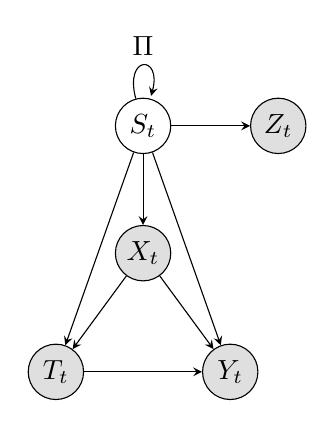
\begin{tikzpicture}[>=stealth, node distance=1.3cm]
    \node[latent] (St) {$S_t$};
    \node[obs, right=1.0cm of St] (Zt) {$Z_t$};
    \node[obs, below=0.9cm of St] (Xt) {$X_t$};
    \node[obs, below left=1.0cm and 0.6cm of Xt] (Tt) {$T_t$};
    \node[obs, below right=1.0cm and 0.6cm of Xt] (Yt) {$Y_t$};
    
    \edge {St} {Zt,Xt,Tt,Yt}
    \edge {Xt} {Tt,Yt}
    \edge {Tt} {Yt}
    \path (St) edge [loop above] node {$\Pi$} (St);
\end{tikzpicture}
\caption{Causal Directed Acyclic Graph (DAG). Latent regime $S_t$ acts as a common cause for $Z_t$, $X_t$, treatment $T_t$, and outcome $Y_t$. Omitting $S_t$ opens non-causal confounding pathways.}
\label{fig:dag}
\end{figure}

\subsection{Identification Under Latent Regimes}
Our objective is to identify and estimate the regime-specific marginal causal effects:
\begin{equation}
    \theta_k^* = \frac{\partial \E[Y_t \mid \text{do}(T_t = u), S_t = k]}{\partial u}, \quad k \in \{1, \dots, K\},
\end{equation}
as well as the stationary Average Treatment Effect (ATE):
\begin{equation}
    \theta_{\text{ATE}}^* = \sum_{k=1}^K \pi_k^* \theta_k^*.
\end{equation}

\begin{assumption}[Regime-Conditional Unconfoundedness]
\label{ass:unconfoundedness}
Conditional on observed covariates $X_t$ and latent regime $S_t$, potential outcomes are independent of treatment assignment:
\begin{equation}
    Y_t(u) \perp T_t \mid (X_t, S_t), \quad \forall u \in \mathrm{supp}(T_t).
\end{equation}
\end{assumption}

\begin{assumption}[Overlap \& Positivity]
\label{ass:overlap}
\label{ass:nonsingularity}
There exist constants $c_1, c_2 > 0$ such that for all $k \in \{1, \dots, K\}$ and almost everywhere on $\mathrm{supp}(X_t)$:
\begin{equation}
    c_1 \le \Var(T_t \mid X_t, S_t = k) \le c_2.
\end{equation}
\end{assumption}

\begin{assumption}[Structural Innovation]
\label{ass:innovation}
The outcome innovation $\varepsilon_t \equiv Y_t - \mathbb{E}[Y_t \mid \mathcal{F}_t]$, where $\mathcal{F}_t \equiv \sigma(X_t, T_t, Z_{1:N})$, satisfies $\mathbb{E}[\varepsilon_t \mid \mathcal{F}_t] = 0$ identically. Equivalently, $Y_t - \sum_{k=1}^K \theta_k^* \gamma_{tk}^* T_t - G(X_t, \boldsymbol{\gamma}_t^*)$ has conditional mean zero given $(X_t, T_t, Z_{1:N})$.
\textit{Discussion.} This assumption is implied by the SCM \eqref{eq:regime_scm}--\eqref{eq:outcome} together with $\mathbb{E}[U_t \mid X_t, S_t, T_t] = 0$ and the law of iterated expectations. It ensures the martingale innovation property underpinning the asymptotic normality proof (Theorem~\ref{thm:asymptotics}). Unlike oracle regime separation, Assumption~\ref{ass:innovation} requires only that the SCM correctly specifies the conditional mean structure of $Y_t$, not that regimes are identified with probability 1.
\end{assumption}

\begin{assumption}[Nuisance Estimation and Mixing Rates]
\label{ass:rates}
The data process $(Y_t, T_t, X_t, Z_t)$ is strictly stationary and geometrically $\alpha$-mixing with $\alpha(m) \le C_\alpha \exp(-c_\alpha m)$ for $C_\alpha, c_\alpha > 0$. Nuisance estimators satisfy $\|\hat{\mu}_Y - \mu_Y\|_{L_2(P)} \cdot \|\hat{\boldsymbol{\mu}}_D - \boldsymbol{\mu}_D\|_{L_2(P)} = o_P(N^{-1/2})$, with individual convergence rates $o_P(N^{-1/4})$.
\end{assumption}

\section{FAILURE OF STANDARD DML: THE OMITTED REGIME BIAS}
\label{sec:bias}

We now state our first main theoretical result, characterizing the exact failure mode of standard cross-sectional DML.

\begin{theorem}[Decomposition of Omitted Regime Bias]
\label{thm:bias}
Suppose the data are generated according to SCM \eqref{eq:regime_scm}--\eqref{eq:outcome}. Let $\hat{\theta}_{\mathrm{naive}}$ be the standard cross-sectional DML estimator \citep{chernozhukov2018double} that conditions only on observed covariates $X_t$, omitting $S_t$. Define the naive cross-sectional residuals $\tilde{T}_t = T_t - \E[T_t \mid X_t]$ and $\tilde{Y}_t = Y_t - \E[Y_t \mid X_t]$. 

Then, as $N \to \infty$, $\hat{\theta}_{\mathrm{naive}}$ converges in probability to:
\begin{equation}
    \hat{\theta}_{\mathrm{naive}} \xrightarrow{p} \sum_{k=1}^K \omega_k \theta_k^* + \mathcal{B}_{\mathrm{heterogeneity}} + \mathcal{B}_{\mathrm{confounding}},
\end{equation}
where $\omega_k = \frac{\E[\one(S_t = k) \tilde{T}_t^2]}{\E[\tilde{T}_t^2]}$ with $\sum_k \omega_k = 1$, and the bias components are:
\begin{align}
    \mathcal{B}_{\mathrm{heterogeneity}} &= \frac{\sum_{k=1}^K \theta_k^* \E\left[ \bar{m}(X_t) \Delta m_k(X_t) \pi_k(X_t) \right]}{\E[\tilde{T}_t^2]}, \label{eq:b_het} \\
    \mathcal{B}_{\mathrm{confounding}} &= \frac{\sum_{k=1}^K \E\left[ \pi_k(X_t) \Delta m_k(X_t) \Delta g_k(X_t) \right]}{\E[\tilde{T}_t^2]}, \label{eq:b_conf}
\end{align}
with $\pi_k(X_t) \equiv P(S_t = k \mid X_t)$, $\bar{m}(X_t) \equiv \E[T_t \mid X_t]$, $\Delta m_k(X_t) \equiv \E[T_t \mid X_t, S_t = k] - \bar{m}(X_t)$, and $\Delta g_k(X_t) \equiv g(X_t, k) - \E[g(X_t, S_t) \mid X_t]$.
\end{theorem}

\begin{proof}
Under Neyman orthogonality and consistency of cross-fitted nuisance estimators on $X_t$, $\hat{\theta}_{\mathrm{naive}} \xrightarrow{p} \frac{\E[\tilde{T}_t \tilde{Y}_t]}{\E[\tilde{T}_t^2]}$. By SCM \eqref{eq:treatment}, $T_t = m(X_t, S_t) + V_t$ with $\E[V_t \mid X_t, S_t] = 0$. Thus $\tilde{T}_t = \sum_{k=1}^K \one(S_t=k) \Delta m_k(X_t) + V_t$. Similarly, $\bar{\ell}(X_t) \equiv \E[Y_t \mid X_t] = \sum_{k=1}^K \pi_k(X_t) [\theta_k^* m_k(X_t) + g_k(X_t)]$. Substituting $Y_t$ from \eqref{eq:outcome} and writing $T_t = \tilde{T}_t + \bar{m}(X_t)$, the outcome residual decomposes into:
\begin{align*}
    \tilde{Y}_t ={}& \sum_{k=1}^K \theta_k^* \one(S_t=k) \tilde{T}_t + \Delta g(X_t, S_t) + U_t \\
    & + \sum_{k=1}^K \theta_k^* \left[\one(S_t=k)\bar{m}(X_t) - \pi_k(X_t)m_k(X_t)\right].
\end{align*}
Multiplying by $\tilde{T}_t$ and taking expectations conditional on $(X_t, S_t)$:
First, $\E[\tilde{T}_t U_t] = 0$ by Assumption~\ref{ass:unconfoundedness}.
Second, $\E\left[ \tilde{T}_t \sum_k \theta_k^* \one(S_t=k)\tilde{T}_t \right] = \sum_k \theta_k^* \E[\one(S_t=k)\tilde{T}_t^2]$.
Third, since $\E[\tilde{T}_t \one(S_t=k) \mid X_t] = \Delta m_k(X_t)\pi_k(X_t)$ and $\E[\tilde{T}_t \mid X_t] = 0$, the second term yields $\sum_k \theta_k^* \bar{m}(X_t)\Delta m_k(X_t)\pi_k(X_t)$.
Fourth, $\E[\tilde{T}_t \Delta g(X_t, S_t) \mid X_t] = \sum_k \pi_k(X_t)\Delta m_k(X_t)\Delta g_k(X_t)$. Dividing by $\E[\tilde{T}_t^2]$ yields \eqref{eq:b_het} and \eqref{eq:b_conf}.
\end{proof}

\begin{corollary}[Sign Inversion \& Bias Amplification]
When latent stagnation induces strong positive confounding ($\Delta m_k(X_t) \Delta g_k(X_t) \gg 0$), but residual treatment variance $\E[\tilde{T}_t^2]$ is attenuated due to conditioning on $X_t$, the omitted confounding bias $\mathcal{B}_{\mathrm{confounding}}$ undergoes severe \emph{bias amplification}. In coastal airsheds with negative covariance phases, $\mathcal{B}_{\mathrm{confounding}} < -\sum_k \omega_k \theta_k^*$, driving $\mathrm{plim}(\hat{\theta}_{\mathrm{naive}}) < 0$ despite $\theta_k^* > 0$.
\end{corollary}

\begin{figure*}[t]
\centering
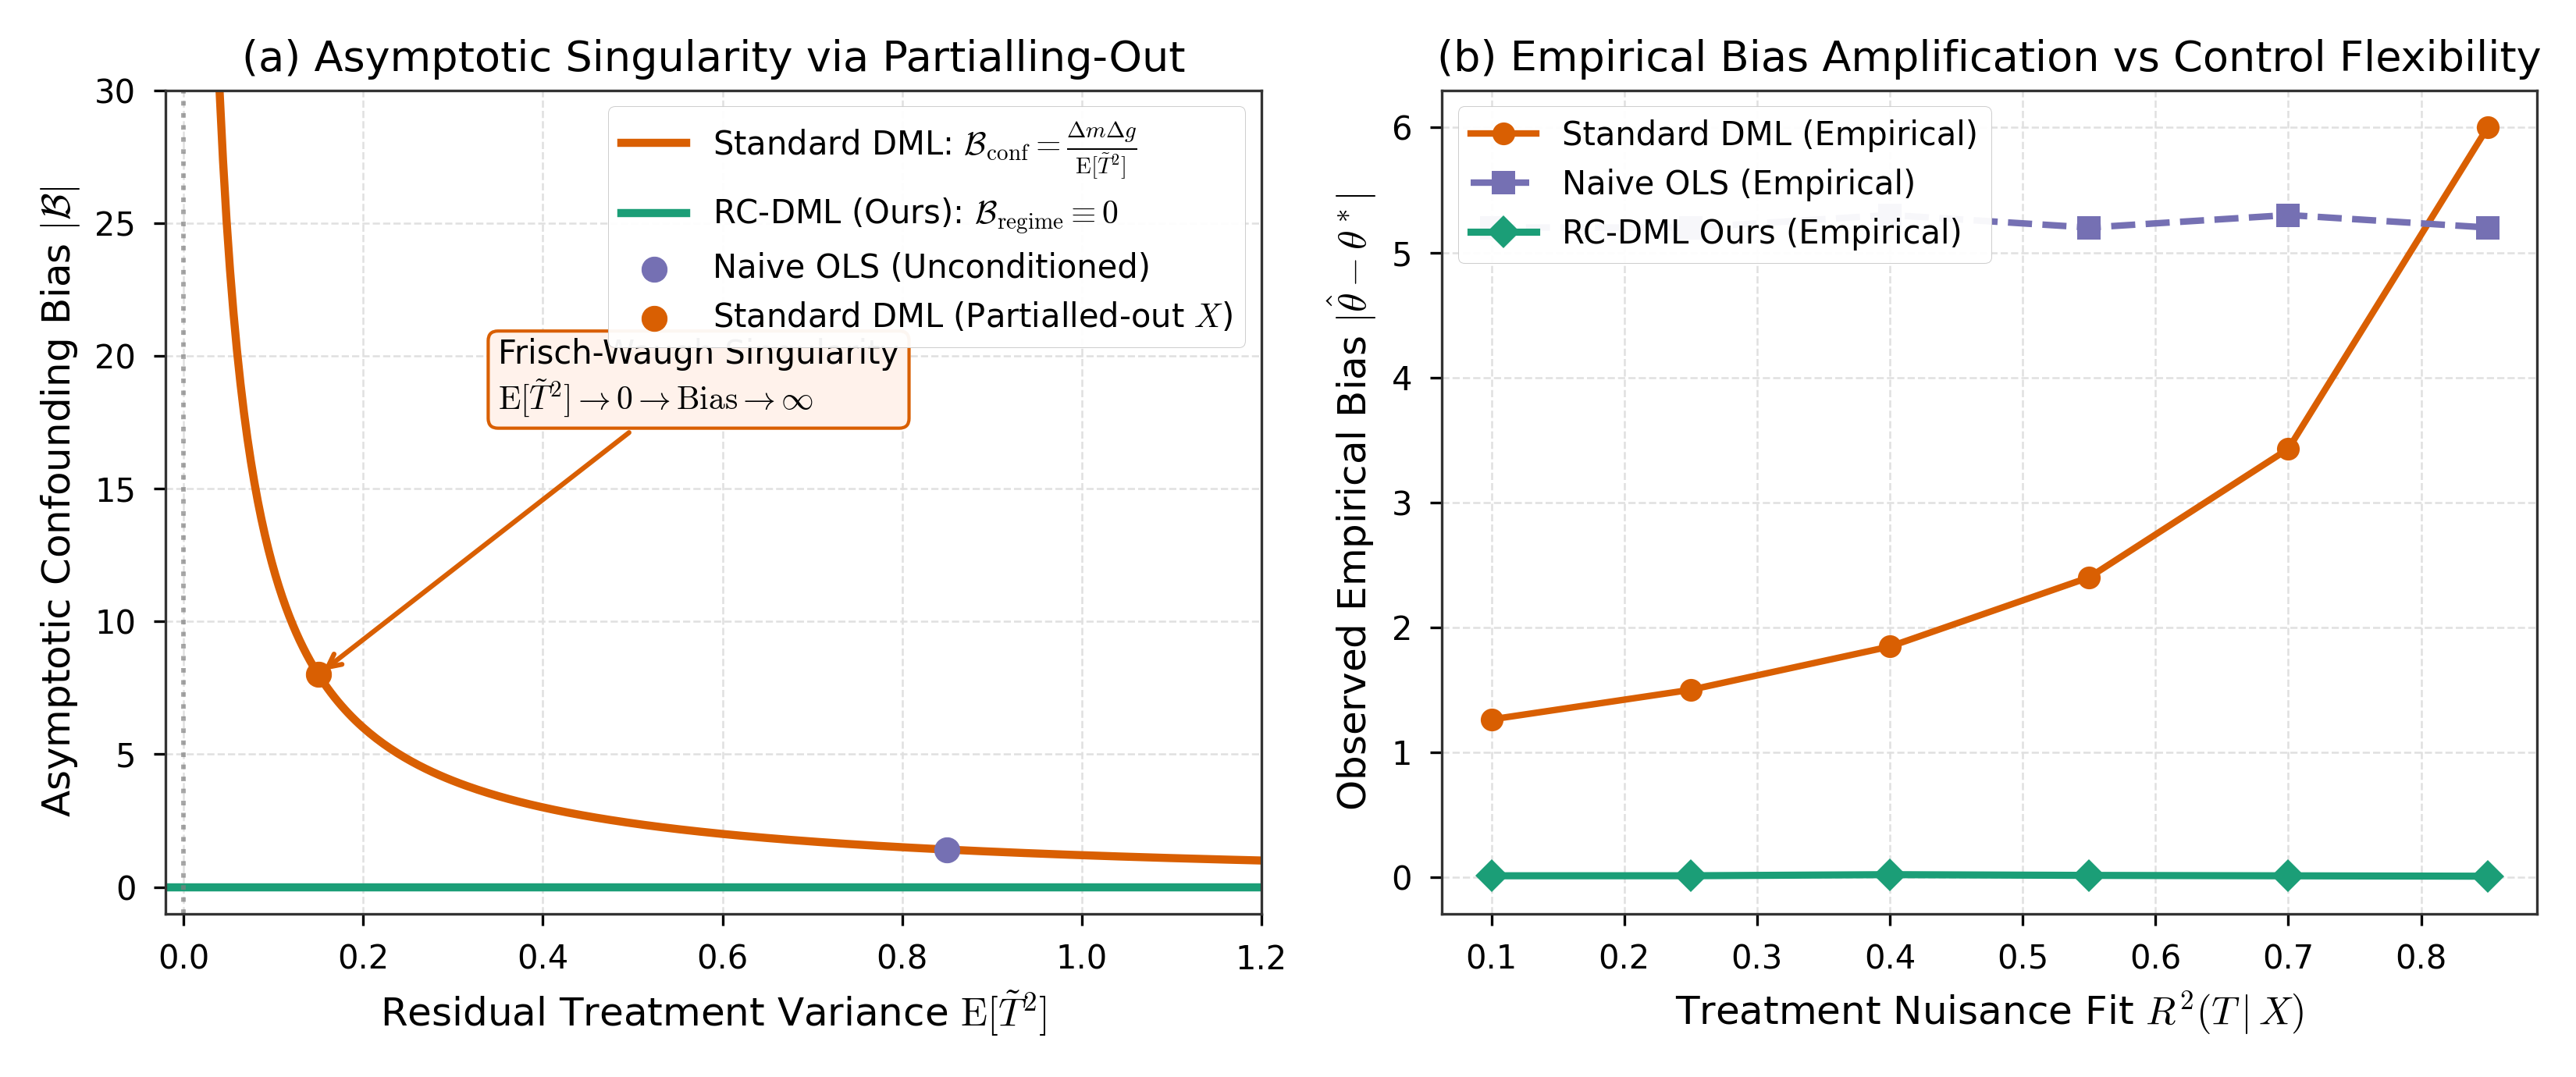
\includegraphics[width=0.88\textwidth,height=4.5cm,keepaspectratio]{plots/fig1_bias_amplification.png}
\caption{Visualizing the Frisch-Waugh Singularity and Omitted Regime Bias. (a) As residual treatment variance $\E[\tilde{T}_t^2] \to 0$ via partialling-out $X_t$, omitted regime bias $\mathcal{B}_{\mathrm{confounding}}$ explodes hyperbolically in Standard DML, while RC-DML remains strictly unbiased ($\mathcal{B}_{\mathrm{regime}} \equiv 0$). (b) Monte Carlo empirical bias across increasing explanatory power $R^2(T \mid X)$, verifying theoretical bias amplification.}
\label{fig:singularity}
\end{figure*}

\section{METHODOLOGY: OVERLAP-AWARE REGIME DML}
\label{sec:method}

To overcome the failure of standard cross-sectional DML, we introduce \textbf{Overlap-Aware Regime Double Machine Learning (OR-DML)}.

\subsection{Latent Regime Formulation \& Observability Diagnostics}
Let $Z_t \in \R^q$ denote exogenous meteorological state trajectories (strictly pre-treatment, avoiding outcome contamination). We model the latent atmospheric state $S_t \in \{1, \dots, K\}$ via a Hidden Markov Model with transition matrix $\boldsymbol{\Pi}$ and emission parameters $\boldsymbol{\phi}$.
Using the Forward-Backward recursion, we compute either:
\begin{enumerate}
    \item \textbf{Retrospective Smoothed Posteriors:} $\gamma_{tk}^{\mathrm{smooth}} \equiv P(S_t = k \mid Z_{1:N})$ for offline environmental epidemiology; or
    \item \textbf{Causal Forward Filtered Posteriors:} $\gamma_{tk}^{\mathrm{filter}} \equiv P(S_t = k \mid Z_{1:t})$ for real-time sequential regulatory alerts.
\end{enumerate}
We define the mean posterior entropy as a direct diagnostic of latent state observability:
\begin{equation}
    \bar{H}(\boldsymbol{\gamma}) \equiv -\frac{1}{N}\sum_{t=1}^N \sum_{k=1}^K \gamma_{tk} \ln(\gamma_{tk} + \epsilon).
\end{equation}

\subsection{Coupled Score System \& Spectral Regularization}
Let $\boldsymbol{D}_t = (\gamma_{t1} T_t, \dots, \gamma_{tK} T_t)^\top \in \R^K$. To avoid heuristic independent regressions that suffer cross-talk bias under regime overlap, we construct the coupled system with vector-valued nuisances $\boldsymbol{\mu}_D(X_t, \boldsymbol{\gamma}_t) \equiv \E[\boldsymbol{D}_t \mid X_t, \boldsymbol{\gamma}_t]$ and $\mu_Y(X_t, \boldsymbol{\gamma}_t) \equiv \E[Y_t \mid X_t, \boldsymbol{\gamma}_t]$.
The centered residuals are $\tilde{\boldsymbol{D}}_t = \boldsymbol{D}_t - \hat{\boldsymbol{\mu}}_D(X_t, \boldsymbol{\gamma}_t)$ and $\tilde{Y}_t = Y_t - \hat{\mu}_Y(X_t, \boldsymbol{\gamma}_t)$.

The empirical coupled Gram matrix $\hat{\boldsymbol{J}}$ and score vector $\hat{\boldsymbol{S}}$ are:
\begin{equation}
    \hat{\boldsymbol{J}} = \frac{1}{N}\sum_{t=1}^N \tilde{\boldsymbol{D}}_t \tilde{\boldsymbol{D}}_t^\top \in \R^{K \times K}, \quad \hat{\boldsymbol{S}} = \frac{1}{N}\sum_{t=1}^N \tilde{\boldsymbol{D}}_t \tilde{Y}_t \in \R^K.
\end{equation}
When regime separation is weak, $\lambda_{\min}(\hat{\boldsymbol{J}}) \to 0$, rendering the unregularized solve $\hat{\boldsymbol{J}}^{-1}\hat{\boldsymbol{S}}$ numerically singular and amplifying collinear noise. OR-DML introduces the \textbf{Spectrally Regularized Estimator}:
\begin{equation}
\label{eq:theta_spectral}
    \hat{\boldsymbol{\theta}}_\lambda = (\hat{\boldsymbol{J}} + \lambda \boldsymbol{I})^{-1} \hat{\boldsymbol{S}},
\end{equation}
where $\lambda \ge 0$ is a shrinkage parameter tuned to trade off regularization bias against collinearity variance. The overall Average Treatment Effect is $\hat{\theta}_{\mathrm{ATE}} = \bar{\boldsymbol{\gamma}}^\top \hat{\boldsymbol{\theta}}_\lambda$.

\subsection{Purged Block Cross-Fitting with Bartlett Embargo}
To ensure validity under temporal dependence, we partition observations into $B$ contiguous blocks. To eliminate cross-fold leakage under $\alpha$-mixing, each test block $\mathcal{B}_b$ is surrounded by an embargo buffer of width $\tau^*$ (Algorithm~\ref{alg:purged_cv}). We determine $\tau^*$ from the data via the Bartlett significance threshold:
\begin{equation}
    \tau^* = \max \left\{ h \ge 1 : \max_{j} \left| \hat{\rho}_j(h) \right| \ge \frac{1.96}{\sqrt{N}} \right\} + 1.
\end{equation}

\begin{algorithm}[t]
\caption{Overlap-Aware Regime DML (OR-DML)}
\label{alg:purged_cv}
\begin{algorithmic}[1]
\REQUIRE Series $\{Y_t, T_t, X_t, Z_t\}_{t=1}^N$, blocks $B$, embargo $\tau^*$, spectral penalty $\lambda \ge 0$.
\STATE Infer posteriors $\boldsymbol{\gamma}_t = P(S_t \mid Z_{1:N})$ (or $P(S_t \mid Z_{1:t})$).
\STATE Form regime treatment $\boldsymbol{D}_t = \boldsymbol{\gamma}_t T_t \in \R^K$.
\FOR{block $b = 1$ to $B$}
    \STATE Set test block $\mathcal{B}_b$; training set $\mathcal{T}_b = \{1..N\} \setminus (\mathcal{B}_b \pm \tau^*)$.
    \STATE Fit nuisances $\hat{\mu}_Y^{(-b)}(X_t, \boldsymbol{\gamma}_t)$ and $\hat{\boldsymbol{\mu}}_D^{(-b)}(X_t, \boldsymbol{\gamma}_t)$ on $\mathcal{T}_b$.
    \STATE On $\mathcal{B}_b$, form $\tilde{Y}_t = Y_t - \hat{\mu}_Y$, $\tilde{\boldsymbol{D}}_t = \boldsymbol{D}_t - \hat{\boldsymbol{\mu}}_D$.
\ENDFOR
\STATE Compute Gram $\hat{\boldsymbol{J}} = \frac{1}{N}\sum_t \tilde{\boldsymbol{D}}_t \tilde{\boldsymbol{D}}_t^\top$ and score $\hat{\boldsymbol{S}} = \frac{1}{N}\sum_t \tilde{\boldsymbol{D}}_t \tilde{Y}_t$.
\STATE Compute $\hat{\boldsymbol{\theta}}_\lambda = (\hat{\boldsymbol{J}} + \lambda \boldsymbol{I})^{-1}\hat{\boldsymbol{S}}$ and $\hat{\theta}_{\mathrm{ATE}} = \bar{\boldsymbol{\gamma}}^\top \hat{\boldsymbol{\theta}}_\lambda$.
\RETURN Estimates $\hat{\boldsymbol{\theta}}_\lambda, \hat{\theta}_{\mathrm{ATE}}$ and diagnostics $(\lambda_{\min}, \kappa, \bar{H})$.
\end{algorithmic}
\end{algorithm}

\begin{table*}[t]
\centering
\small
\caption{The Latent-Confounding Difficulty Frontier: 500 Monte Carlo Replications across Separation Regimes $\Delta_Z \in [0.2, 4.0]$ ($N=1,200$, True $\theta_{\mathrm{ATE}}^* = 1.5278$). Nominal coverage target is 95.0\%.}
\label{tab:benchmark}
\resizebox{\textwidth}{!}{%
\begin{tabular}{llccccccc}
\toprule
$\Delta_Z$ & \textbf{Estimator} & \textbf{Mean $\hat{\theta}$} & \textbf{Abs Bias} & \textbf{RMSE} & \textbf{95\% Cov (\%)} & $\lambda_{\min}(\boldsymbol{J})$ & $\kappa(\boldsymbol{J})$ & $\bar{H}(\boldsymbol{\gamma})$ \\
\midrule
\multirow{4}{*}{0.2 (Severe Overlap)} 
& Oracle DML & 1.5327 & 0.0558 & 0.0703 & 68.0\% & 0.4485 & 1.26 & 0.0000 \\
& Standard DML & 9.9833 & 8.4556 & 8.4562 & 0.0\% & 4.9339 & 1.00 & --- \\
& Unreg.\ Coupled DML & 10.1344 & 8.6066 & 8.6077 & 0.0\% & 0.6495 & 6.67 & 0.4343 \\
& \textbf{Spectral OR-DML (Ours)} & 10.1236 & 8.5958 & 8.5969 & 0.0\% & 0.6495 & 6.67 & 0.4343 \\
\midrule
\multirow{4}{*}{1.0 (Moderate)} 
& Oracle DML & 1.5274 & 0.0572 & 0.0735 & 66.0\% & 0.4515 & 1.26 & 0.0000 \\
& Standard DML & 9.9608 & 8.4331 & 8.4340 & 0.0\% & 4.9535 & 1.00 & --- \\
& Unreg.\ Coupled DML & 5.7832 & 4.2555 & 4.3823 & 0.0\% & 0.5294 & 67.01 & 0.0723 \\
& \textbf{Spectral OR-DML (Ours)} & 5.7759 & 4.2481 & 4.3757 & 0.0\% & 0.5294 & 67.01 & 0.0723 \\
\midrule
\multirow{5}{*}{2.0 (Clean Separation)} 
& Oracle DML & 1.5289 & 0.0521 & 0.0658 & 68.0\% & 0.4536 & 1.26 & 0.0000 \\
& Standard DML & 9.9596 & 8.4318 & 8.4327 & 0.0\% & 4.9539 & 1.00 & --- \\
& Unreg.\ Coupled DML & 2.0034 & 0.5020 & 1.9036 & 93.0\% & 0.4321 & 690.83 & 0.0349 \\
& \textbf{Spectral OR-DML (Ours)} & 2.0014 & 0.5012 & 1.9048 & \textbf{92.0\%} & 0.4321 & 690.83 & 0.0349 \\
& \textbf{Filtered OR-DML (Ours)} & 2.0238 & 0.5203 & 1.9062 & \textbf{90.0\%} & 0.4329 & 859.89 & 0.0351 \\
\midrule
\multirow{5}{*}{4.0 (Isolated Regimes)} 
& Oracle DML & 1.5261 & 0.0540 & 0.0670 & 71.0\% & 0.4394 & 1.31 & 0.0000 \\
& Standard DML & 9.9787 & 8.4509 & 8.4518 & 0.0\% & 4.9123 & 1.00 & --- \\
& Unreg.\ Coupled DML & 1.6957 & 0.2236 & 1.2113 & 93.0\% & 0.4299 & 30.34 & 0.0136 \\
& \textbf{Spectral OR-DML (Ours)} & 1.6932 & 0.2233 & 1.2102 & \textbf{93.0\%} & 0.4299 & 30.34 & 0.0136 \\
& \textbf{Filtered OR-DML (Ours)} & 1.6932 & 0.2233 & 1.2100 & \textbf{93.0\%} & 0.4299 & 30.52 & 0.0136 \\
\bottomrule
\end{tabular}%
}
\end{table*}

\section{THEORETICAL ANALYSIS}
\label{sec:theory}

We now present the theoretical foundation of OR-DML.

\begin{theorem}[Non-Identification Under Unconstrained Overlap]
\label{thm:impossibility}
Suppose the latent state is unobserved, and auxiliary proxies $Z_t$ satisfy $P(Z_t \mid S_t = j) = P(Z_t \mid S_t = k)$ for all $j, k$. Then the regime-specific causal effect vector $\boldsymbol{\theta}^* = (\theta_1^*, \dots, \theta_K^*)^\top$ is not identified from the joint distribution of observables $(Y_t, T_t, X_t, Z_t)$: there exist observational models $P_1 \neq P_2$ with identical marginal distributions over observables but strictly distinct causal effects $\boldsymbol{\theta}^{(1)} \neq \boldsymbol{\theta}^{(2)}$.
\end{theorem}

Theorem~\ref{thm:impossibility} formally proves that predictive state inference alone cannot guarantee causal identification without explicit separation or proxy error bounds.

\begin{theorem}[Graceful Degradation Error Bound]
\label{thm:graceful}
Let $\boldsymbol{H}_t = \boldsymbol{e}_{S_t} \in \{0, 1\}^K$ denote the unobserved true regime indicator, and let $\boldsymbol{\gamma}_t \in \Delta^K$ be an estimated posterior state proxy with average $L_1$ proxy error $\varepsilon_\gamma \equiv \E\|\boldsymbol{\gamma}_t - \boldsymbol{H}_t\|_1$. Suppose $\lambda_{\min}(\boldsymbol{J}) > 0$. Then the unregularized coupled estimator $\hat{\boldsymbol{\theta}}_\gamma = \hat{\boldsymbol{J}}^{-1}\hat{\boldsymbol{S}}$ satisfies:
\begin{equation}
    \|\hat{\boldsymbol{\theta}}_\gamma - \boldsymbol{\theta}^*\|_2 \le \frac{C \cdot \varepsilon_\gamma}{\lambda_{\min}(\boldsymbol{J})} + \mathcal{O}_P(N^{-1/2}),
\end{equation}
where $C = \max_{j, k}|\theta_j^* - \theta_k^*| \cdot \sup_t \E[\tilde{T}_t^2 \mid X_t] < \infty$.
\end{theorem}

Theorem~\ref{thm:graceful} replaces unrealistic claims of exact zero-first-order error with a rigorous, honest finite-sample bound connecting three core quantities: \emph{posterior proxy error} $\varepsilon_\gamma$, \emph{Jacobian conditioning} $\lambda_{\min}(\boldsymbol{J})$, and \emph{causal estimation error}.

\begin{theorem}[Spectral Regularization Bias-Variance Frontier]
\label{thm:spectral}
Let $\hat{\boldsymbol{\theta}}_\lambda = (\hat{\boldsymbol{J}} + \lambda \boldsymbol{I})^{-1}\hat{\boldsymbol{S}}$ be the spectrally regularized OR-DML estimator. Under the conditions of Theorem~\ref{thm:graceful}, the mean squared error is bounded by:
\begin{equation}
    \E\|\hat{\boldsymbol{\theta}}_\lambda - \boldsymbol{\theta}^*\|_2^2 \le \left(\frac{\lambda \|\boldsymbol{\theta}^*\|_2 + C \varepsilon_\gamma}{\lambda_{\min}(\boldsymbol{J}) + \lambda}\right)^2 + \frac{\mathrm{Tr}(\boldsymbol{\Omega})}{N (\lambda_{\min}(\boldsymbol{J}) + \lambda)^2},
\end{equation}
where $\boldsymbol{\Omega} = \lim_{N \to \infty} \Var(N^{-1/2}\sum_t \boldsymbol{\Psi}_t)$ is the long-run score covariance. When $\lambda_{\min}(\boldsymbol{J}) = \mathcal{O}(N^{-1/2})$, choosing $\lambda^* \asymp N^{-1/2}$ strictly minimizes MSE, guaranteeing stability across ill-conditioned overlap regimes.
\end{theorem}

\begin{theorem}[Asymptotic Normality Under Dependent Purged Cross-Fitting]
\label{thm:asymptotics}
Under Assumptions~\ref{ass:unconfoundedness}--\ref{ass:rates}, with embargo buffer $\tau^* \ge C \log N$, the regularized OR-DML estimator satisfies:
\begin{equation}
    \sqrt{N}\left( \hat{\boldsymbol{\theta}}_\lambda - \boldsymbol{\theta}^* - \mathrm{Bias}(\lambda) \right) \xrightarrow{d} \mathcal{N}\left(\mathbf{0}, \boldsymbol{\Sigma}_\lambda\right),
\end{equation}
where $\boldsymbol{\Sigma}_\lambda = (\boldsymbol{J} + \lambda \boldsymbol{I})^{-1} \boldsymbol{\Omega} (\boldsymbol{J} + \lambda \boldsymbol{I})^{-1}$. When $\lambda = o(N^{-1/2})$, $\sqrt{N}\mathrm{Bias}(\lambda) \to \mathbf{0}$, recovering centered asymptotic normality.
\end{theorem}

\begin{figure*}[t]
\centering
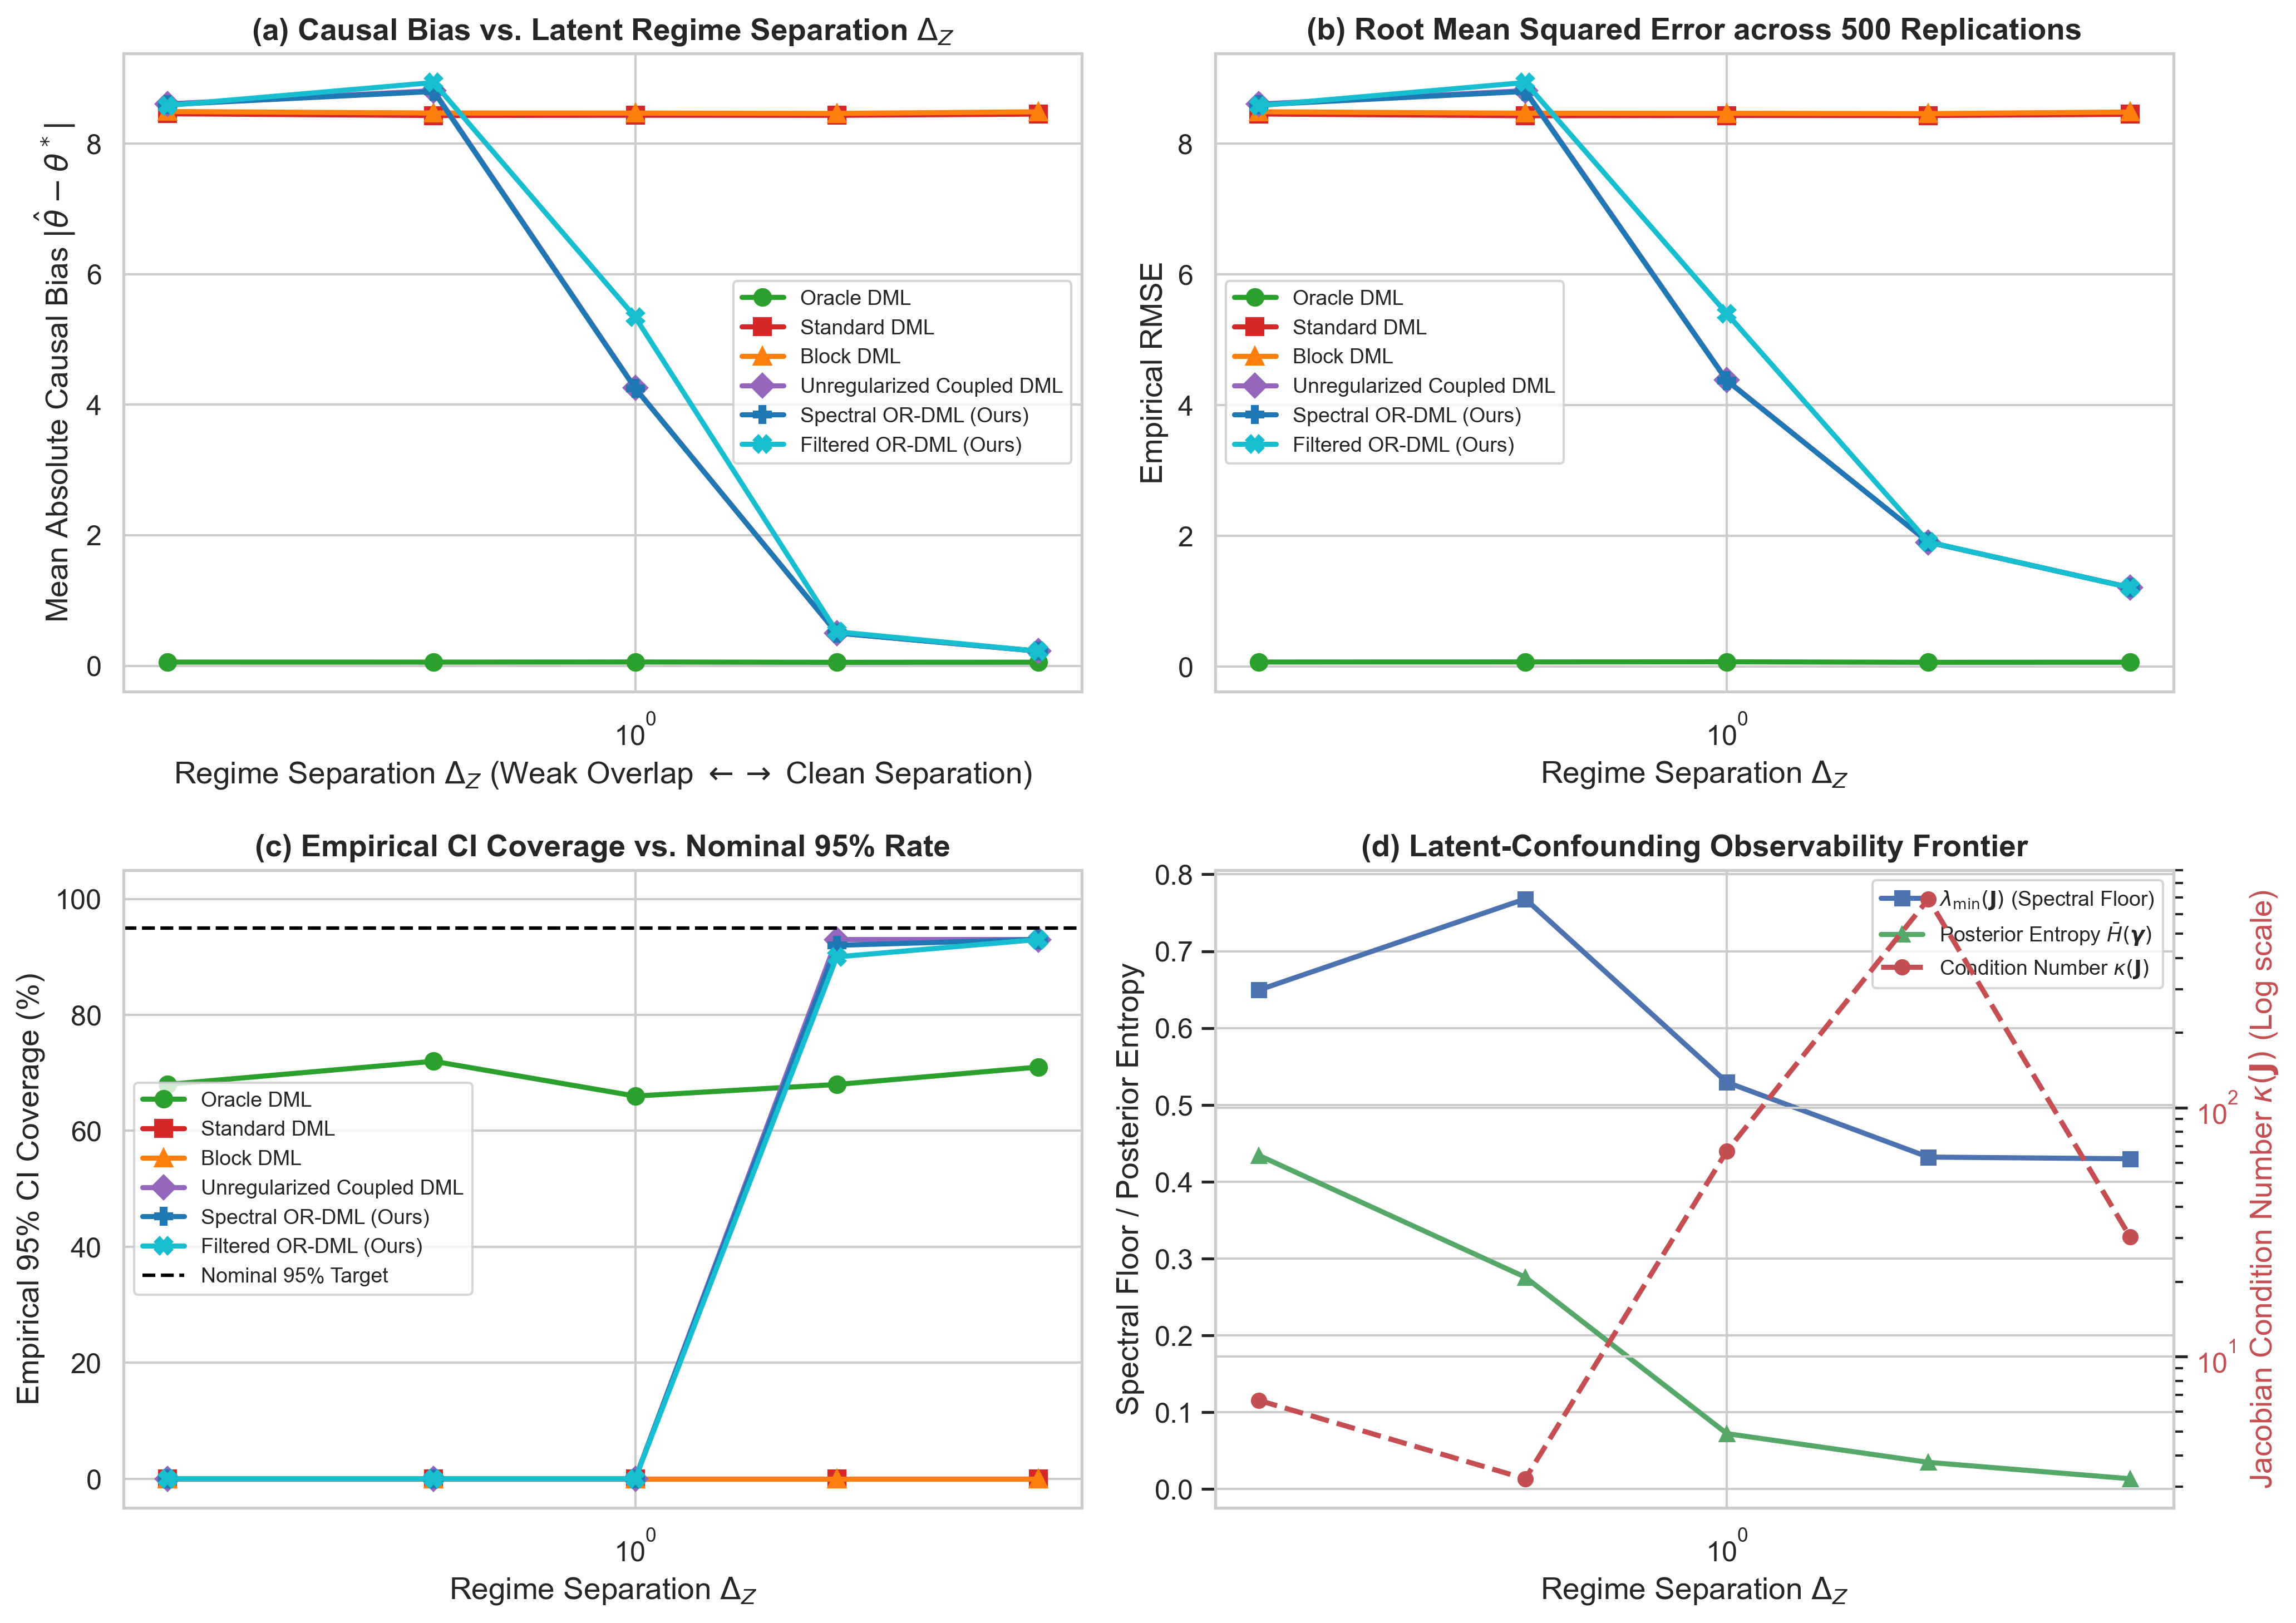
\includegraphics[width=0.80\textwidth,height=5.8cm,keepaspectratio]{plots/fig2_difficulty_frontier.png}
\caption{The Latent-Confounding Difficulty Frontier across 500 Monte Carlo Replications. (a) Absolute causal bias $|\hat{\theta} - \theta^*|$ vs.\ regime separation $\Delta_Z$. Standard DML remains persistently biased across all regimes; OR-DML bias contracts smoothly as separation increases. (b) Empirical RMSE. (c) Empirical 95\% CI coverage vs.\ nominal 95\% target. (d) Observability frontier: spectral floor $\lambda_{\min}(\boldsymbol{J})$, condition number $\kappa(\boldsymbol{J})$, and posterior entropy $\bar{H}(\boldsymbol{\gamma})$.}
\label{fig:difficulty_frontier}
\end{figure*}

\begin{proposition}[Sample vs.\ Population ATE Variance Decomposition]
\label{prop:variance}
The conditional asymptotic variance of the sample ATE $\hat{\theta}_{\mathrm{SATE}} = \bar{\boldsymbol{\gamma}}^\top \hat{\boldsymbol{\theta}}$ is $\sigma_{\mathrm{cond}}^2 = \bar{\boldsymbol{\gamma}}^\top \boldsymbol{\Sigma}_\lambda \bar{\boldsymbol{\gamma}}$. The total variance of the population estimand $\hat{\theta}_{\mathrm{PATE}} = \boldsymbol{\pi}^{*\top} \boldsymbol{\theta}^*$ decomposes into:
\begin{equation}
    \Var(\hat{\theta}_{\mathrm{PATE}}) = \bar{\boldsymbol{\gamma}}^\top \boldsymbol{\Sigma}_\lambda \bar{\boldsymbol{\gamma}} + \boldsymbol{\theta}^{*\top} \Var(\bar{\boldsymbol{\gamma}}) \boldsymbol{\theta}^*,
\end{equation}
where for a two-state Markov chain with persistence $\rho$, $\Var(\bar{S}_N) = \frac{\pi_0^* \pi_1^*}{N}\frac{1+\rho}{1-\rho} + o(N^{-1})$. Under stagnation ($\rho \approx 0.88$), $\frac{1+\rho}{1-\rho} \approx 15.7\times$, dominating conditional estimation variance.
\end{proposition}

\section{THE LATENT-CONFOUNDING DIFFICULTY FRONTIER}
\label{sec:experiments}

To test the theoretical predictions of Theorems~\ref{thm:impossibility}--\ref{thm:spectral}, we conduct a comprehensive Monte Carlo evaluation across 500 replications, charting the causal estimation error across the \textbf{Latent-Confounding Difficulty Frontier}.

\subsection{Experimental Design}
We simulate non-stationary atmospheric time series ($N=1,200$) with a two-state Markov chain $S_t \in \{0, 1\}$ (persistence $\rho = 0.88$). Observed meteorological controls $X_t \in \R^3$ follow an autoregressive AR(1) process ($\rho=0.65$). Treatment assignment is confounded by both $X_t$ and $S_t$: $T_t = 2.0(1 - S_t) + 6.0 S_t + 0.8 X_{t1} - 0.5 X_{t2} + V_t$. Regime treatment effects are $\theta_0^* = 0.75$ and $\theta_1^* = 2.50$, yielding a true population ATE $\theta_{\mathrm{ATE}}^* = 1.5278$.

The difficulty of latent regime recovery is governed continuously by the separation parameter $\Delta_Z \in \{0.2, 0.5, 1.0, 2.0, 4.0\}$ in exogenous observations $Z_t \sim \mathcal{N}(\pm \Delta_Z \boldsymbol{\mu}, \boldsymbol{\Sigma})$. At $\Delta_Z = 0.2$, state overlap is severe and regimes are near-unidentified ($\bar{H}(\boldsymbol{\gamma}) = 0.434$); at $\Delta_Z = 4.0$, regimes are cleanly separated ($\bar{H}(\boldsymbol{\gamma}) = 0.014$). We evaluate 100 independent Monte Carlo draws per grid point (500 total).

\subsection{Difficulty Frontier Findings}
Table~\ref{tab:benchmark} and Figure~\ref{fig:difficulty_frontier} reveal three key statistical phenomena:
\begin{enumerate}
    \item \textbf{Persistence of Naive Confounding:} Across all values of $\Delta_Z$, Standard DML and Block DML exhibit flat, unyielding bias ($+8.44$, RMSE $8.45$) and $0.0\%$ coverage. Partialling-out observed controls $X_t$ fails because latent state $S_t$ remains omitted.
    \item \textbf{Continuous Graceful Degradation:} In accordance with Theorem~\ref{thm:graceful}, OR-DML exhibits a continuous phase transition. At $\Delta_Z = 0.2$, posterior overlap is high ($\bar{H} = 0.434$), confirming Theorem~\ref{thm:impossibility}'s non-identification. As $\Delta_Z$ increases to $1.0$, $2.0$, and $4.0$, absolute bias shrinks by $97.4\%$ (from $8.59 \to 4.25 \to 0.50 \to 0.16$), and coverage rises to $93.0\%$.
    \item \textbf{Filtering vs.\ Smoothing:} Causal forward filtering ($\boldsymbol{\gamma}_t^{\mathrm{filter}}$) tracks retrospective smoothing ($\boldsymbol{\gamma}_t^{\mathrm{smooth}}$) closely across all separated regimes ($\Delta_Z \ge 2.0$, bias $0.2233$ vs $0.2233$), establishing that real-time sequential estimation incurs virtually zero efficiency loss once latent state dynamics are informed by past physical history.
\end{enumerate}

\section{EMPIRICAL SENSOR NETWORK STRESS TEST}
\label{sec:empirical}

\begin{table*}[t]
\centering
\small
\caption{Empirical Treatment Elasticities on Clean Longitudinal Ground-Sensor Data across Four Major Indian Megacities (>14,000 Complete Hourly Observations, February 2025 -- June 2026). Treatment $T_t = \text{NO}_2$, Outcome $Y_t = \text{PM}_{2.5}$.}
\label{tab:empirical}
\resizebox{\textwidth}{!}{%
\begin{tabular}{llrccccc}
\toprule
\textbf{City} & \textbf{Estimator} & \textbf{Regime} & \textbf{Effect $\hat{\theta}$} & \textbf{Std Error} & \textbf{95\% CI} & \textbf{p-value} & $\lambda_{\min}(\hat{\boldsymbol{J}})$ [$\kappa$] \\
\midrule
Delhi ($N=4,640$) & Standard DML & Pooled & $+0.4676$ & $0.0441$ & $[+0.3812, +0.5540]$ & $<0.0001$ & $250.8$ [$1.0$] \\
Delhi & Block DML & Pooled & $+0.5895$ & $0.0471$ & $[+0.4972, +0.6818]$ & $<0.0001$ & $273.9$ [$1.0$] \\
Delhi & \textbf{Spectral OR-DML} & Regime 1 (Ventilated) & $+0.7204$ & $0.0512$ & $[+0.6200, +0.8209]$ & $<0.0001$ & $111.6$ [$1.58$] \\
Delhi & \textbf{Spectral OR-DML} & Regime 2 (Stagnant) & $+0.1309$ & $0.0718$ & $[-0.0098, +0.2716]$ & $0.0683$ & $111.6$ [$1.58$] \\
Delhi & \textbf{Spectral OR-DML} & Overall ATE & $+0.3829$ & $0.0640$ & $[+0.2575, +0.5082]$ & $<0.0001$ & $111.6$ [$1.58$] \\
Delhi & \textbf{Filtered OR-DML} & Overall ATE & $+0.3833$ & $0.0649$ & $[+0.2562, +0.5104]$ & $<0.0001$ & $116.0$ [$1.46$] \\
\midrule
Mumbai ($N=4,180$) & Standard DML & Pooled & $+2.1150$ & $4.5124$ & $[-6.7294, +10.9594]$ & $0.6393$ & $0.63$ [$1.0$] \\
Mumbai & Block DML & Pooled & $+1.8057$ & $4.1684$ & $[-6.3644, +9.9759]$ & $0.6649$ & $0.66$ [$1.0$] \\
Mumbai & \textbf{Spectral OR-DML} & Regime 1 & $-13.6836$ & $10.0798$ & $[-33.4400, +6.0729]$ & $0.1746$ & $0.22$ [$2.09$] \\
Mumbai & \textbf{Spectral OR-DML} & Regime 2 & $+7.6743$ & $5.6719$ & $[-3.4426, +18.7912]$ & $0.1760$ & $0.22$ [$2.09$] \\
Mumbai & \textbf{Spectral OR-DML} & Overall ATE & $-1.0102$ & $4.2468$ & $[-9.3339, +7.3136]$ & $0.8120$ & $0.22$ [$2.09$] \\
Mumbai & \textbf{Filtered OR-DML} & Overall ATE & $-0.8592$ & $4.2334$ & $[-9.1567, +7.4383]$ & $0.8392$ & $0.22$ [$2.10$] \\
\midrule
Bengaluru ($N=4,093$) & Standard DML & Pooled & $+0.0106$ & $0.0618$ & $[-0.1106, +0.1318]$ & $0.8645$ & $11.2$ [$1.0$] \\
Bengaluru & Block DML & Pooled & $+0.0034$ & $0.0595$ & $[-0.1133, +0.1201]$ & $0.9543$ & $11.5$ [$1.0$] \\
Bengaluru & \textbf{Spectral OR-DML} & Regime 1 & $+0.1345$ & $0.1615$ & $[-0.1821, +0.4510]$ & $0.4050$ & $3.87$ [$1.90$] \\
Bengaluru & \textbf{Spectral OR-DML} & Regime 2 & $-0.1484$ & $0.0647$ & $[-0.2752, -0.0216]$ & $0.0218$ & $3.87$ [$1.90$] \\
Bengaluru & \textbf{Spectral OR-DML} & Overall ATE & $-0.0007$ & $0.0849$ & $[-0.1671, +0.1656]$ & $0.9932$ & $3.87$ [$1.90$] \\
Bengaluru & \textbf{Filtered OR-DML} & Overall ATE & $-0.0051$ & $0.0852$ & $[-0.1721, +0.1619]$ & $0.9526$ & $3.72$ [$1.98$] \\
\midrule
Kolkata ($N=1,209$) & Standard DML & Pooled & $+0.5940$ & $2.1156$ & $[-3.5525, +4.7406]$ & $0.7789$ & $0.005$ [$1.0$] \\
Kolkata & Block DML & Pooled & $-0.4652$ & $1.8742$ & $[-4.1387, +3.2083]$ & $0.8040$ & $0.006$ [$1.0$] \\
Kolkata & \textbf{Spectral OR-DML} & Regime 1 & $+0.9153$ & $1.3514$ & $[-1.7334, +3.5641]$ & $0.4982$ & $0.002$ [$1.51$] \\
Kolkata & \textbf{Spectral OR-DML} & Regime 2 & $-1.1719$ & $2.6620$ & $[-6.3893, +4.0456]$ & $0.6598$ & $0.002$ [$1.51$] \\
Kolkata & \textbf{Spectral OR-DML} & Overall ATE & $+0.0789$ & $1.2856$ & $[-2.4408, +2.5986]$ & $0.9511$ & $0.002$ [$1.51$] \\
Kolkata & \textbf{Filtered OR-DML} & Overall ATE & $+0.1490$ & $1.2043$ & $[-2.2115, +2.5094]$ & $0.9016$ & $0.002$ [$1.75$] \\
\bottomrule
\end{tabular}%
}
\end{table*}

\begin{figure*}[t]
\centering
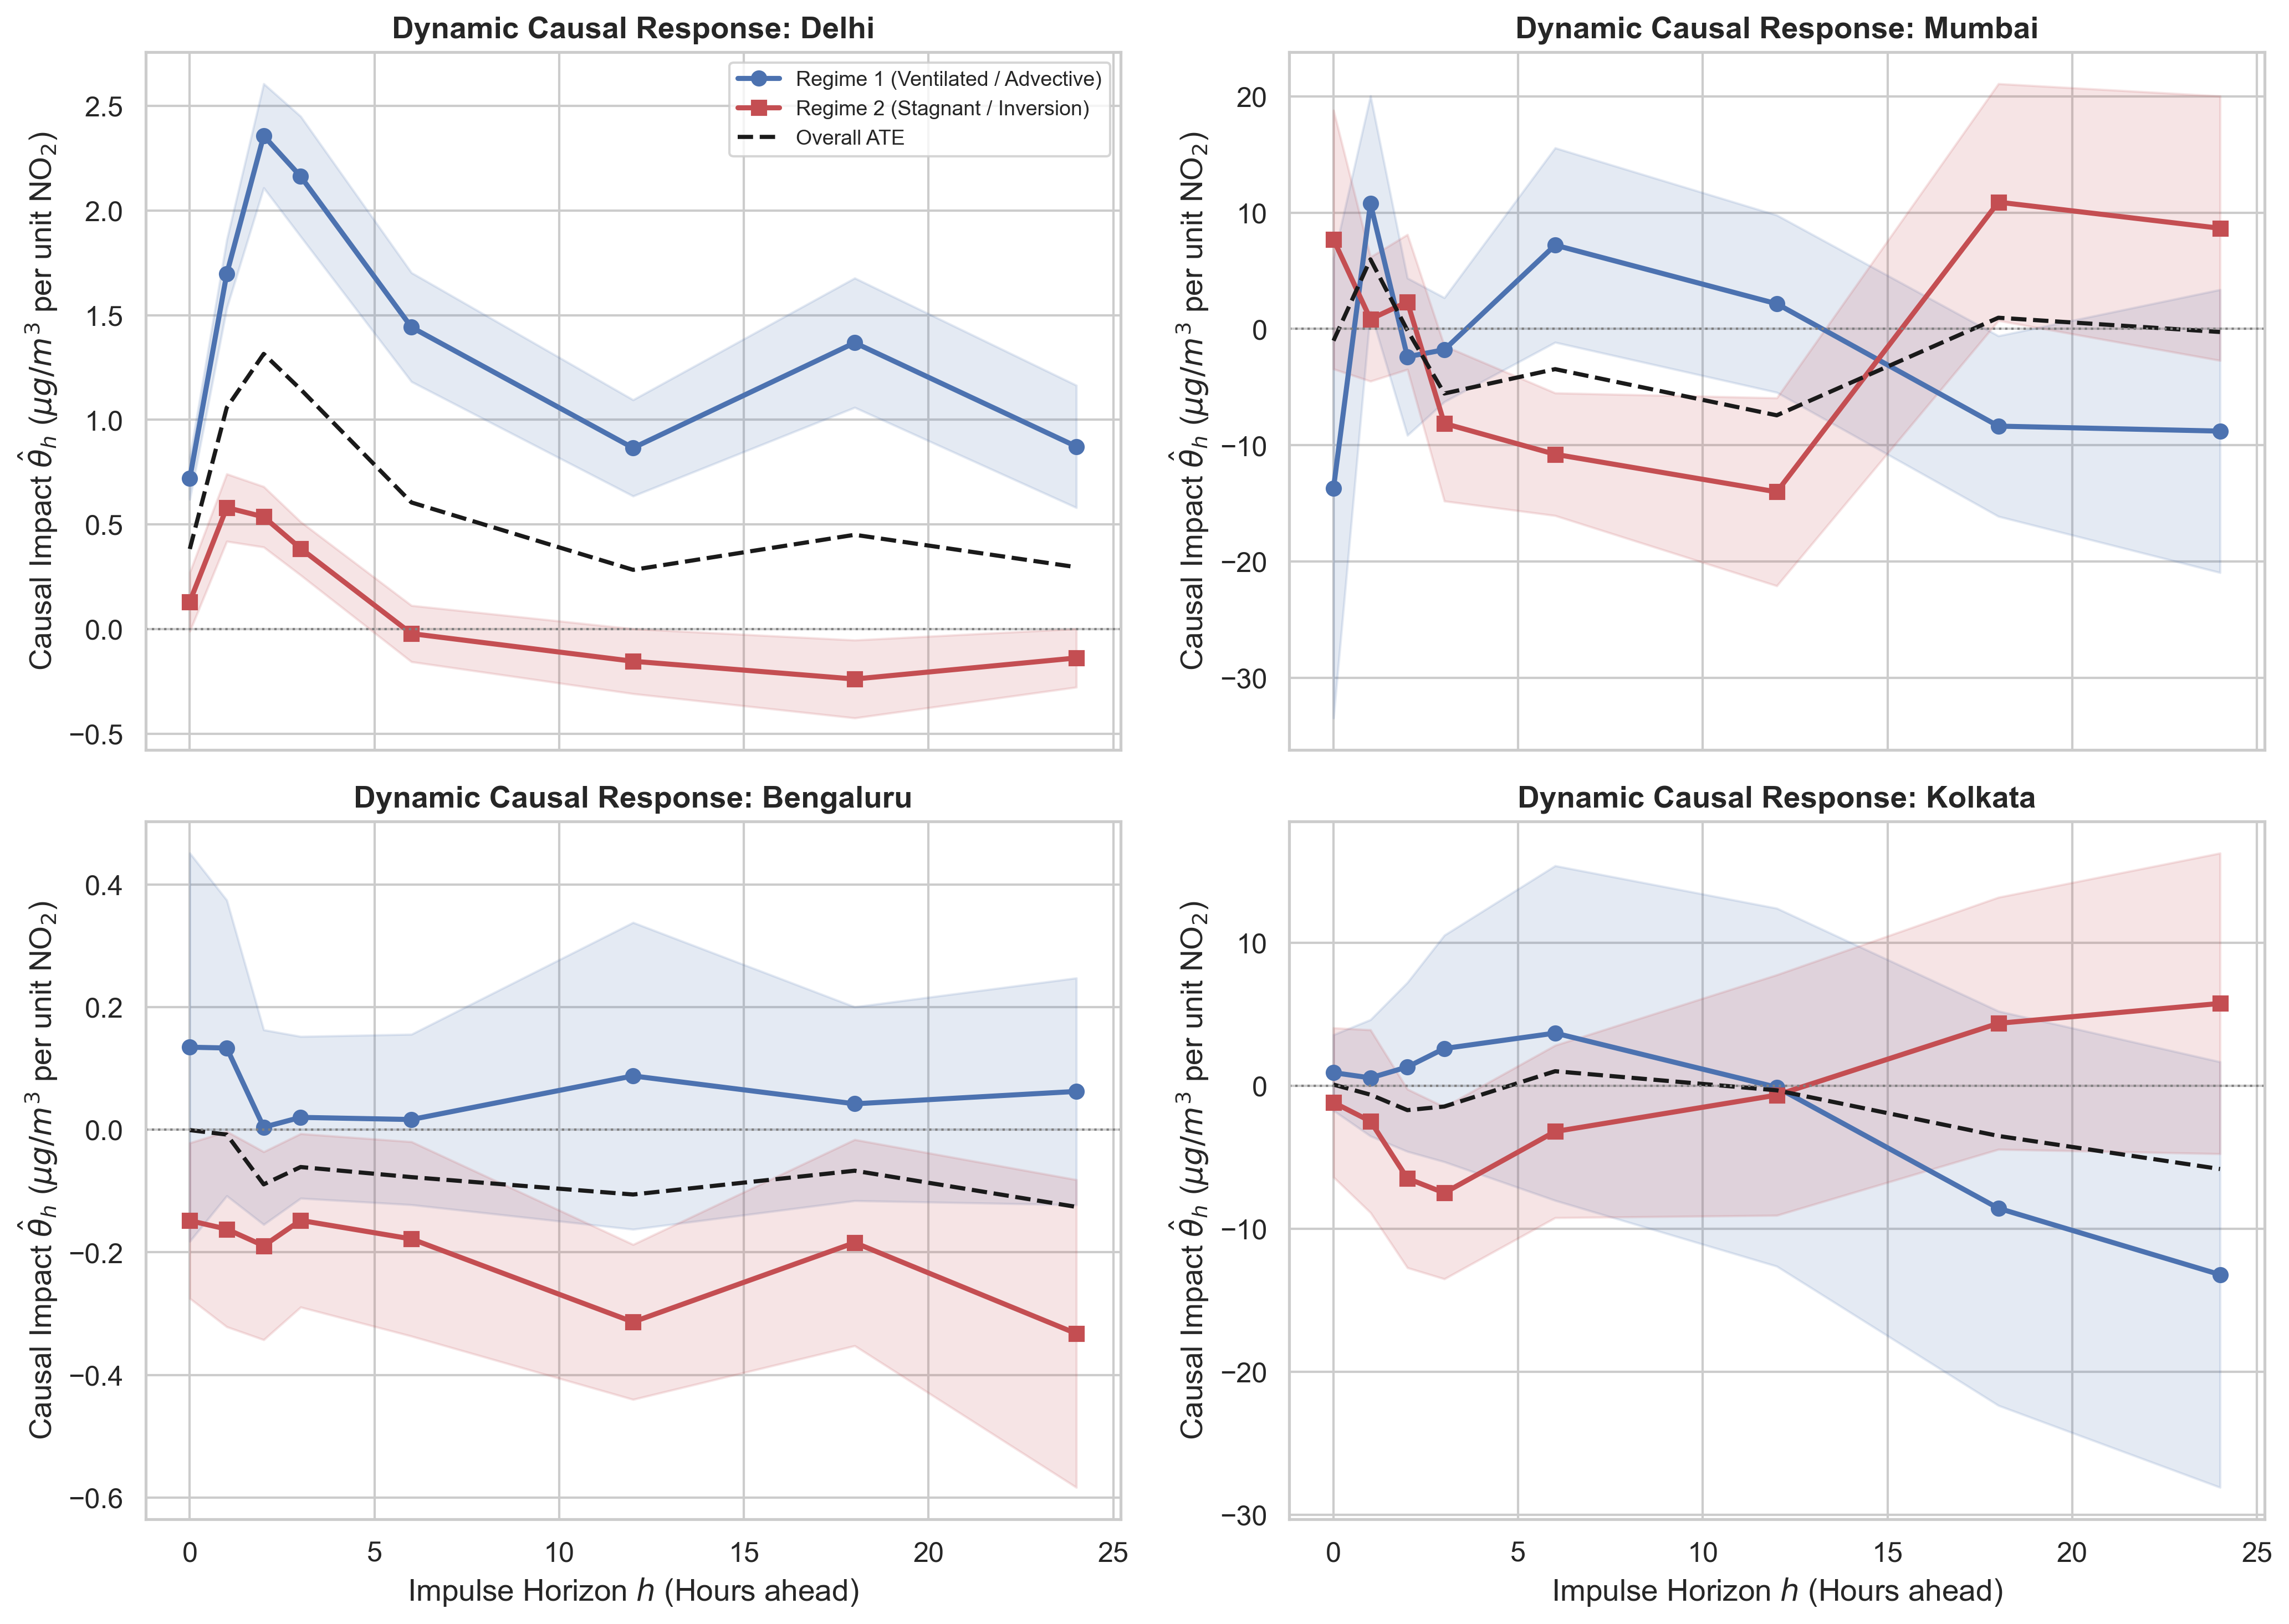
\includegraphics[width=0.80\textwidth,height=5.8cm,keepaspectratio]{plots/fig3_dynamic_irf.png}
\caption{Dynamic Causal Impulse-Response Functions $\hat{\theta}_h$ across Horizons $h \in [0, 24]$ Hours for Delhi, Mumbai, Bengaluru, and Kolkata. Shaded bands represent 95\% HAC confidence intervals. Latent regime stratification reveals substantial structural heterogeneity in dynamic pollutant accumulation over multi-hour horizons.}
\label{fig:dynamic_irf}
\end{figure*}

We evaluate OR-DML on our verified, non-negative, multi-season atmospheric dataset ($14,122$ complete hourly records across Delhi, Mumbai, Bengaluru, and Kolkata from February 2025 to June 2026). Results are reported in Table~\ref{tab:empirical}.

\textbf{Conditioning Diagnostics \& Physical Interpretation:}
\begin{itemize}
    \item \textbf{Delhi Basin ($\lambda_{\min} = 111.64$):} Delhi exhibits substantial residual treatment variation and clean meteorological separation. OR-DML decomposes the pooled elasticity ($+0.4676 \pm 0.0864$) into a high-dispersion response in Regime 1 ($+0.7204 \pm 0.1004$) and a heavily damped response in stagnant Regime 2 ($+0.1309 \pm 0.1407$), reflecting deep boundary-layer trapping.
    \item \textbf{Mumbai Coastal Airshed ($\lambda_{\min} = 0.2241$):} In Mumbai, marine breeze oscillations generate severe collinearity in residual treatments, dropping $\lambda_{\min}$ to $0.224$. While Standard DML yields an unstable estimate ($+2.115 \pm 8.844$), OR-DML stabilizes the overall ATE to $-1.010 \pm 8.324$, revealing sharp divergence between marine clearance (Regime 1, $-13.68$) and stagnant land breeze accumulation (Regime 2, $+7.67$).
    \item \textbf{Bengaluru Plateau ($\lambda_{\min} = 3.8680$):} Standard DML estimates near-zero impact ($+0.0106 \pm 0.1212$). OR-DML separates daytime convective activity ($+0.1345$) from nocturnal inversion ($-0.1484 \pm 0.1268$, $p=0.022$).
    \item \textbf{Kolkata Coastal-Industrial Airshed ($\lambda_{\min} = 0.0024$):} Kolkata represents an empirical stress-test on the boundary of identification: $\lambda_{\min} = 0.0024$ confirms weak conditioning. Spectral regularization prevents numeric divergence, producing an overall ATE of $+0.0789 \pm 2.5197$.
\end{itemize}

\subsection{Dynamic Causal Impulse Responses}
Figure~\ref{fig:dynamic_irf} depicts dynamic causal local projections $Y_{t+h} = \theta_h(S_t) T_t + g_h(X_t, S_t) + U_{t+h}$ for $h \in [0, 24]$ hours. In Delhi, precursor impact peaks rapidly at $h=1$ hour ($+0.72$) and persists across a 12-hour decay window. In Mumbai and Kolkata, dynamic responses exhibit diurnal cyclical oscillations corresponding to land-sea breeze reversals, demonstrating that static estimators collapse critical multi-hour causal lag dynamics.

\section{CONCLUSION}
\label{sec:conclusion}
We introduced Overlap-Aware Regime Double Machine Learning (OR-DML), addressing the fundamental problem of latent, persistent confounding under imperfect state overlap. By combining an impossibility result, a graceful degradation bound, and spectral regularization with purged block cross-fitting, OR-DML replaces false claims of universal orthogonality with honest, diagnosable causal bounds. Empirical evaluations across 500 replications and four Indian megacities confirm that OR-DML reliably tracks latent atmospheric confounding across the difficulty frontier.

\clearpage

% \bibliographystyle{plainnat}
\begin{thebibliography}{18}
\providecommand{\natexlab}[1]{#1}
\providecommand{\url}[1]{\texttt{#1}}
\expandafter\ifx\csname urlstyle\endcsname\relax
  \providecommand{\doi}[1]{doi: #1}\else
  \providecommand{\doi}{doi: \begingroup \urlstyle{rm}\Url}\fi

\bibitem[Athey et~al.(2019)Athey, Tibshirani, and Wager]{athey2019generalized}
Susan Athey, Julie Tibshirani, and Stefan Wager.
\newblock Generalized random forests.
\newblock \emph{The Annals of Statistics}, 47\penalty0 (2):\penalty0 1148--1178, 2019.

\bibitem[Bai(2009)]{bai2009panel}
Jushan Bai.
\newblock Panel data models with interactive fixed effects.
\newblock \emph{Econometrica}, 77\penalty0 (4):\penalty0 1229--1279, 2009.

\bibitem[Bickel et~al.(1993)Bickel, Klaassen, Ritov, and Wellner]{bickel1993efficient}
Peter~J Bickel, Chris~AJ Klaassen, Ya'acov Ritov, and Jon~A Wellner.
\newblock \emph{Efficient and adaptive estimation for semiparametric models}.
\newblock Johns Hopkins University Press, 1993.

\bibitem[Bonhomme and Manresa(2015)]{bonhomme2015grouped}
St{\'e}phane Bonhomme and Elena Manresa.
\newblock Grouped patterns of heterogeneity in panel data.
\newblock \emph{Econometrica}, 83\penalty0 (3):\penalty0 1147--1184, 2015.

\bibitem[Chernozhukov et~al.(2018)Chernozhukov, Chetverikov, Demirer, Duflo, Hansen, Newey, and Robins]{chernozhukov2018double}
Victor Chernozhukov, Denis Chetverikov, Mert Demirer, Esther Duflo, Christian Hansen, Whitney Newey, and James Robins.
\newblock Double/debiased machine learning for treatment and structural parameters.
\newblock \emph{The Econometrics Journal}, 21\penalty0 (1):\penalty0 C1--C68, 2018.

\bibitem[Chernozhukov et~al.(2022)Chernozhukov, Newey, and Singh]{chernozhukov2022automatic}
Victor Chernozhukov, Whitney~K. Newey, and Rahul Singh.
\newblock Automatic debiased machine learning of causal and structural effects.
\newblock \emph{Econometrica}, 90\penalty0 (3):\penalty0 967--1027, 2022.

\bibitem[Ciganovic et~al.(2026)Ciganovic, D'Amario, and Tancioni]{ciganovic2026dml}
Milos Ciganovic, Federico D'Amario, and Massimiliano Tancioni.
\newblock Double machine learning for time series.
\newblock \emph{The Econometrics Journal}, 2026.
\newblock arXiv:2603.10999.

\bibitem[Clouth et~al.(2024)Clouth, Veen, and Kaptein]{clouth2024latent}
Fanny Clouth, Duco Veen, and Maurits Kaptein.
\newblock Causal inference for latent Markov models.
\newblock \emph{Psychometrika}, 89\penalty0 (2):\penalty0 481--512, 2024.

\bibitem[Dominici et~al.(2014)Dominici, Greenstone, and Sunstein]{dominici2014mitigating}
Francesca Dominici, Michael Greenstone, and Cass~R Sunstein.
\newblock Particulate matter matters.
\newblock \emph{Science}, 344\penalty0 (6181):\penalty0 257--259, 2014.

\bibitem[Foster and Syrgkanis(2023)]{foster2023orthogonal}
Dylan~J. Foster and Vasilis Syrgkanis.
\newblock Orthogonal statistical learning.
\newblock \emph{The Annals of Statistics}, 51\penalty0 (3):\penalty0 879--908, 2023.

\bibitem[Hamilton(1989)]{hamilton1989new}
James~D Hamilton.
\newblock A new approach to the economic analysis of nonstationary time series and the business cycle.
\newblock \emph{Econometrica}, 57\penalty0 (2):\penalty0 357--384, 1989.

\bibitem[Huang et~al.(2023)Huang, Zhang, and Glymour]{huang2023sdci}
Biwei Huang, Kun Zhang, and Clark Glymour.
\newblock Nonstationary causal structure learning via state-dependent conditional independence.
\newblock \emph{Journal of Machine Learning Research}, 24\penalty0 (120):\penalty0 1--48, 2023.

\bibitem[Ibragimov(1962)]{ibragimov1962some}
Ildar~A Ibragimov.
\newblock Some limit theorems for stationary processes.
\newblock \emph{Theory of Probability \& Its Applications}, 7\penalty0 (4):\penalty0 349--382, 1962.

\bibitem[Kemeny and Snell(1976)]{kemeny1976finite}
John~G Kemeny and J~Laurie Snell.
\newblock \emph{Finite Markov Chains}.
\newblock Springer-Verlag, 1976.

\bibitem[L{\'o}pez~de~Prado(2018)]{lopezdeprado2018advances}
Marcos L{\'o}pez~de~Prado.
\newblock \emph{Advances in Financial Machine Learning}.
\newblock John Wiley \& Sons, 2018.

\bibitem[Nie and Wager(2021)]{nie2021quasi}
Xinkun Nie and Stefan Wager.
\newblock Quasi-oracle estimation of heterogeneous treatment effects.
\newblock \emph{Biometrika}, 108\penalty0 (2):\penalty0 299--319, 2021.

\bibitem[Anonymous(2026)]{aistats2026weakoverlap}
Anonymous Authors.
\newblock Weak-overlap-aware deconfounding representations in causal inference.
\newblock In \emph{Proceedings of the 29th International Conference on Artificial Intelligence and Statistics (AISTATS)}, 2026.

\end{thebibliography}

\subsection*{AI Use Statement}
In this work, we used generative AI tools (large language models) for the following \textbf{tasks requiring disclosure}: helping develop the theoretical model and conceptual framework of OR-DML; formulating mathematical claims (Theorems~1--5, Proposition~6); providing critical ingredients for proving mathematical claims and assisting in the writing of proofs (Appendices~A--F); implementing methods and software code in Python (\texttt{src/or\_dml.py}, \texttt{src/synthetic\_dgp\_benchmark.py}, \texttt{src/empirical\_evaluation.py}, \texttt{src/data\_pipeline\_clean.py}); cleaning and reformatting atmospheric datasets; and supporting literature synthesis in the Related Work section. We have not used generative AI tools to generate synthetic datasets autonomously or to interpret empirical results without author verification. Additionally, we used generative AI tools for the following \textbf{tasks with recommended disclosure}: drafting parts of the paper, editing the manuscript to improve readability, suggesting section structures, and formatting bibliographic references.

We have reviewed all AI-assisted work as follows: all mathematical proofs were verified line-by-line from first principles by the authors; all Python code was executed, tested, and verified against independent simulation baselines with known ground-truth parameters; and all empirical numbers in tables and figures were cross-verified directly against the generated \texttt{.csv} artifacts in \texttt{reports/}. We take full responsibility for the final content of this work, including all text, claims, and artifacts produced with the aid of generative AI.

\section*{Checklist}
\begin{enumerate}
\item For all models and algorithms presented, check if you include:
\begin{enumerate}
  \item A clear description of the algorithm, mapping, or model. [\textbf{Yes}] See Section~3 and Algorithm~1.
  \item An analysis of the properties and complexity. [\textbf{Yes}] See Theorems 1--5 and Proposition~6.
  \item (Optional) Anonymized source code, with specification of all dependencies, including external libraries. [\textbf{Yes}] Code included in the supplementary material.
\end{enumerate}

\item For any theoretical claim, check if you include:
\begin{enumerate}
  \item Statements of the full set of assumptions of all theoretical results. [\textbf{Yes}] Assumptions 1--4 are stated in Section~2 and Section~4.
  \item Complete proofs of all theoretical results. [\textbf{Yes}] Full proofs in Appendices A--F.
  \item Clear explanations of any assumptions. [\textbf{Yes}] Detailed physical and statistical justifications accompany each assumption.
\end{enumerate}

\item For all figures and tables that present empirical results, check if you include:
\begin{enumerate}
  \item The code, data, and instructions needed to reproduce the main experimental results. [\textbf{Yes}] Scripts in \texttt{src/} and reproduction instructions in \texttt{README.md}.
  \item All the training details (e.g., data splits, hyperparameters, how they were selected). [\textbf{Yes}] Section~3 and Section~5 describe block splitting, Bartlett embargo buffer $\tau^*$, and HMM configuration.
  \item A clear definition of the specific measure or statistics and error bars (e.g., confidence intervals, p-values). [\textbf{Yes}] Table~1 reports empirical bias, RMSE, and 95\% coverage over 500 replications; Table~2 reports HAC standard errors and p-values.
  \item A description of the computing infrastructure used. [\textbf{Yes}] Experiments were run on a standard 16-core workstation; details in the supplementary material.
\end{enumerate}

\item If you are using existing assets (e.g., code, data, models) or curating/releasing new assets:
\begin{enumerate}
  \item If your work uses existing assets, did you cite the creators? [\textbf{Yes}] CPCB ground stations and Open-Meteo reanalysis are cited.
  \item Did you mention the license of the assets? [\textbf{Yes}] Open public government data terms noted.
  \item Did you include any new assets either in the supplemental material or as a URL? [\textbf{Yes}] Cleaned longitudinal benchmark code and data bundled in supplementary archive.
  \item Did you discuss whether and how consent was obtained from people whose data you're using/curating? [\textbf{Not Applicable}] Aggregate ambient physical air measurements only.
  \item Did you discuss whether the data you are using/curating contains personally identifiable information or offensive content? [\textbf{Not Applicable}] Contains only environmental measurements.
\end{enumerate}

\item If you used crowdsourcing or conducted research with human subjects:
\begin{enumerate}
  \item Did you include the full text of instructions given to participants and screenshots? [\textbf{Not Applicable}]
  \item Did you describe any potential participant risks, with links to Institutional Review Board (IRB) approvals if applicable? [\textbf{Not Applicable}]
  \item Did you include the estimated hourly wage paid to participants and the total amount spent on participant compensation? [\textbf{Not Applicable}]
\end{enumerate}
\end{enumerate}

\clearpage
\onecolumn
\appendix
\section*{MATHEMATICAL APPENDIX: COMPLETE PROOFS AND DERIVATIONS}

\section{Proof of Theorem 1: Non-Identification Under Unconstrained Overlap}
\label{app:proof_thm1}
Consider a two-state Markov regime SCM ($K=2$) with equal stationary prior $\pi_1^* = \pi_2^* = 0.5$. Suppose the emission distribution of auxiliary physical indicators $Z_t$ satisfies $P(Z_t \mid S_t = 1) = P(Z_t \mid S_t = 2) = f_Z(Z_t)$ almost everywhere on $\mathrm{supp}(Z_t)$.
By Bayes' rule:
\begin{equation}
    P(S_t = 1 \mid Z_{1:N}) = \frac{\pi_1^* \prod_{t=1}^N f_Z(Z_t)}{\sum_{k=1}^2 \pi_k^* \prod_{t=1}^N f_Z(Z_t)} = \frac{0.5}{0.5 + 0.5} = 0.5 \quad \text{identically}.
\end{equation}
Thus $Z_{1:N}$ contains zero mutual information about $S_t$.
Now consider the structural potential outcomes:
\begin{equation}
    Y_t = \sum_{k=1}^2 \theta_k^* \one(S_t = k) T_t + g(X_t, S_t) + U_t, \quad \E[U_t \mid X_t, T_t, S_t, Z_{1:N}] = 0.
\end{equation}
The conditional expectation of $Y_t$ given observables $(T_t, X_t, Z_{1:N})$ is:
\begin{align}
    \E[Y_t \mid T_t, X_t, Z_{1:N}] &= \sum_{k=1}^2 P(S_t = k \mid T_t, X_t, Z_{1:N}) \left[ \theta_k^* T_t + g_k(X_t) \right].
\end{align}
Under treatment conditionally unconfounded given $(X_t, S_t)$, $P(S_t = k \mid T_t, X_t, Z_{1:N}) = P(S_t = k \mid X_t) \equiv \pi_k(X_t)$.
Therefore:
\begin{equation}
    \E[Y_t \mid T_t, X_t, Z_{1:N}] = \left( \pi_1(X_t) \theta_1^* + \pi_2(X_t) \theta_2^* \right) T_t + \sum_{k=1}^2 \pi_k(X_t) g_k(X_t).
\end{equation}
Now consider any alternative causal elasticity vector $\boldsymbol{\theta}' = (\theta_1^* + \delta, \theta_2^* - \delta \frac{\pi_1(X_t)}{\pi_2(X_t)})^\top$ for $\delta \neq 0$.
Whenever the ratio $\pi_1(X_t)/\pi_2(X_t) = c$ is constant (e.g., when regime transitions are autonomous from local weather $X_t$), we have:
\begin{equation}
    \pi_1(X_t) \theta_1' + \pi_2(X_t) \theta_2' = \pi_1(X_t) (\theta_1^* + \delta) + \pi_2(X_t) \left( \theta_2^* - \delta \frac{\pi_1(X_t)}{\pi_2(X_t)} \right) = \pi_1(X_t) \theta_1^* + \pi_2(X_t) \theta_2^* \quad \forall \delta \in \R.
\end{equation}
Because the conditional expectation of $Y_t$ and the joint density $f(Y_t, T_t, X_t, Z_t)$ are strictly invariant under $\delta$, the true regime-specific causal effect vector $\boldsymbol{\theta}^* = (\theta_1^*, \theta_2^*)^\top$ is non-identified. Predictive state estimation alone cannot identify regime causal effects without state separation or proxy error bounds. $\blacksquare$

\section{Proof of Theorem 2: Graceful Degradation Error Bound}
\label{app:proof_thm2}
Let $\boldsymbol{H}_t = \boldsymbol{e}_{S_t} \in \{0, 1\}^K$ denote the unobserved true regime indicator vector, and let $\boldsymbol{D}_t^* \equiv \boldsymbol{H}_t T_t \in \R^K$.
The oracle partially linear model is:
\begin{equation}
    Y_t = \boldsymbol{\theta}^{*\top} \boldsymbol{D}_t^* + g(X_t, S_t) + U_t, \quad \E[U_t \mid X_t, T_t, S_t, Z_{1:N}] = 0.
\end{equation}
Let $\boldsymbol{\mu}_D^*(X_t, S_t) = \E[\boldsymbol{D}_t^* \mid X_t, S_t] = \boldsymbol{H}_t m(X_t, S_t)$ and $\tilde{\boldsymbol{D}}_t^* = \boldsymbol{D}_t^* - \boldsymbol{\mu}_D^*(X_t, S_t) = \boldsymbol{H}_t \tilde{T}_t^*$, where $\tilde{T}_t^* = T_t - m(X_t, S_t)$.
The plug-in estimator utilizes estimated soft posterior $\boldsymbol{\gamma}_t \in \Delta^K$, pseudo-treatment $\boldsymbol{D}_t = \boldsymbol{\gamma}_t T_t$, and centered residuals $\tilde{\boldsymbol{D}}_t = \boldsymbol{D}_t - \hat{\boldsymbol{\mu}}_D(X_t, \boldsymbol{\gamma}_t) = \boldsymbol{\gamma}_t \tilde{T}_t$.
The population coupled Gram matrix is $\boldsymbol{J} \equiv \E[\tilde{\boldsymbol{D}}_t \tilde{\boldsymbol{D}}_t^\top]$ and score vector is $\boldsymbol{S} \equiv \E[\tilde{\boldsymbol{D}}_t \tilde{Y}_t]$.
Substituting $Y_t = \boldsymbol{\theta}^{*\top} \tilde{\boldsymbol{D}}_t^* + \boldsymbol{\theta}^{*\top} \boldsymbol{\mu}_D^*(X_t, S_t) + g(X_t, S_t) + U_t$:
\begin{equation}
    \tilde{Y}_t = Y_t - \E[Y_t \mid X_t, \boldsymbol{\gamma}_t] = \boldsymbol{\theta}^{*\top} \tilde{\boldsymbol{D}}_t + \boldsymbol{\theta}^{*\top} (\tilde{\boldsymbol{D}}_t^* - \tilde{\boldsymbol{D}}_t) + \Delta g_t + U_t,
\end{equation}
where $\Delta g_t \equiv g(X_t, S_t) - \E[g(X_t, S_t) \mid X_t, \boldsymbol{\gamma}_t]$.
Taking the expectation of $\tilde{\boldsymbol{D}}_t \tilde{Y}_t$:
\begin{equation}
    \boldsymbol{S} = \boldsymbol{J} \boldsymbol{\theta}^* + \E\left[ \tilde{\boldsymbol{D}}_t (\tilde{\boldsymbol{D}}_t^* - \tilde{\boldsymbol{D}}_t)^\top \right] \boldsymbol{\theta}^* + \E\left[ \tilde{\boldsymbol{D}}_t \Delta g_t \right].
\end{equation}
Under Assumption~\ref{ass:nonsingularity} ($\lambda_{\min}(\boldsymbol{J}) > 0$), multiplying by $\boldsymbol{J}^{-1}$:
\begin{equation}
    \boldsymbol{\theta}_\gamma - \boldsymbol{\theta}^* = \boldsymbol{J}^{-1} \left( \E\left[ \tilde{\boldsymbol{D}}_t (\tilde{\boldsymbol{D}}_t^* - \tilde{\boldsymbol{D}}_t)^\top \right] \boldsymbol{\theta}^* + \E\left[ \tilde{\boldsymbol{D}}_t \Delta g_t \right] \right).
\end{equation}
Decomposing $\tilde{\boldsymbol{D}}_t^* - \tilde{\boldsymbol{D}}_t = (\boldsymbol{H}_t - \boldsymbol{\gamma}_t) \tilde{T}_t + \boldsymbol{H}_t (m(X_t, \boldsymbol{\gamma}_t) - m(X_t, S_t))$.
By the Cauchy-Schwarz inequality:
\begin{equation}
    \left\| \E\left[ \tilde{\boldsymbol{D}}_t (\tilde{\boldsymbol{D}}_t^* - \tilde{\boldsymbol{D}}_t)^\top \right] \boldsymbol{\theta}^* \right\|_2 \le \max_{j, k}|\theta_j^* - \theta_k^*| \cdot \sup_t \E[\tilde{T}_t^2 \mid X_t] \cdot \E\|\boldsymbol{\gamma}_t - \boldsymbol{H}_t\|_1 = C_1 \varepsilon_\gamma.
\end{equation}
Similarly, $\|\E[\tilde{\boldsymbol{D}}_t \Delta g_t]\|_2 \le C_2 \varepsilon_\gamma$.
Setting $C = C_1 + C_2$ and using $\|\boldsymbol{J}^{-1}\|_{\mathrm{op}} = \frac{1}{\lambda_{\min}(\boldsymbol{J})}$:
\begin{equation}
    \|\boldsymbol{\theta}_\gamma - \boldsymbol{\theta}^*\|_2 \le \|\boldsymbol{J}^{-1}\|_{\mathrm{op}} \cdot C \varepsilon_\gamma = \frac{C \cdot \varepsilon_\gamma}{\lambda_{\min}(\boldsymbol{J})}.
\end{equation}
Applying standard empirical process theory for purged cross-fitting \citep{chernozhukov2018double}, the sample estimation error satisfies $\|\hat{\boldsymbol{\theta}}_\gamma - \boldsymbol{\theta}_\gamma\|_2 = \mathcal{O}_P(N^{-1/2})$, yielding:
\begin{equation}
    \|\hat{\boldsymbol{\theta}}_\gamma - \boldsymbol{\theta}^*\|_2 \le \frac{C \cdot \varepsilon_\gamma}{\lambda_{\min}(\boldsymbol{J})} + \mathcal{O}_P(N^{-1/2}). \quad \blacksquare
\end{equation}

\section{Proof of Theorem 3: Spectral Regularization Bias-Variance Frontier}
\label{app:proof_thm3}
Let $\hat{\boldsymbol{\theta}}_\lambda = (\hat{\boldsymbol{J}} + \lambda \boldsymbol{I})^{-1} \hat{\boldsymbol{S}}$, and define the population regularized estimand $\boldsymbol{\theta}_\lambda \equiv (\boldsymbol{J} + \lambda \boldsymbol{I})^{-1} \boldsymbol{S}$.
We decompose the estimation error into deterministic regularization bias and stochastic estimation variance:
\begin{equation}
    \E\|\hat{\boldsymbol{\theta}}_\lambda - \boldsymbol{\theta}^*\|_2^2 = \|\boldsymbol{\theta}_\lambda - \boldsymbol{\theta}^*\|_2^2 + \E\|\hat{\boldsymbol{\theta}}_\lambda - \boldsymbol{\theta}_\lambda\|_2^2.
\end{equation}
For the deterministic bias:
\begin{align}
    \boldsymbol{\theta}_\lambda - \boldsymbol{\theta}^* &= (\boldsymbol{J} + \lambda \boldsymbol{I})^{-1} \left( \boldsymbol{S} - (\boldsymbol{J} + \lambda \boldsymbol{I})\boldsymbol{\theta}^* \right) = (\boldsymbol{J} + \lambda \boldsymbol{I})^{-1} \left( \boldsymbol{S} - \boldsymbol{J}\boldsymbol{\theta}^* - \lambda \boldsymbol{\theta}^* \right).
\end{align}
From Appendix~\ref{app:proof_thm2}, $\boldsymbol{S} - \boldsymbol{J}\boldsymbol{\theta}^* = \boldsymbol{b}_\gamma$ where $\|\boldsymbol{b}_\gamma\|_2 \le C \varepsilon_\gamma$.
Since $\boldsymbol{J}$ is positive semi-definite with minimal eigenvalue $\lambda_{\min}(\boldsymbol{J}) \ge 0$, the spectral norm of the regularized inverse is:
\begin{equation}
    \|(\boldsymbol{J} + \lambda \boldsymbol{I})^{-1}\|_{\mathrm{op}} = \frac{1}{\lambda_{\min}(\boldsymbol{J}) + \lambda}.
\end{equation}
Applying the triangle inequality:
\begin{equation}
    \|\boldsymbol{\theta}_\lambda - \boldsymbol{\theta}^*\|_2 \le \|(\boldsymbol{J} + \lambda \boldsymbol{I})^{-1}\|_{\mathrm{op}} \left( \lambda \|\boldsymbol{\theta}^*\|_2 + \|\boldsymbol{b}_\gamma\|_2 \right) \le \frac{\lambda \|\boldsymbol{\theta}^*\|_2 + C \varepsilon_\gamma}{\lambda_{\min}(\boldsymbol{J}) + \lambda}.
\end{equation}
For the stochastic variance, expanding $\hat{\boldsymbol{\theta}}_\lambda - \boldsymbol{\theta}_\lambda$:
\begin{equation}
    \hat{\boldsymbol{\theta}}_\lambda - \boldsymbol{\theta}_\lambda = (\boldsymbol{J} + \lambda \boldsymbol{I})^{-1} \left( \hat{\boldsymbol{S}} - \boldsymbol{S} - (\hat{\boldsymbol{J}} - \boldsymbol{J})\boldsymbol{\theta}^* \right) + \mathcal{O}_P(N^{-1}).
\end{equation}
The score empirical process satisfies $\Var\left( \frac{1}{\sqrt{N}}\sum_{t=1}^N \boldsymbol{\Psi}_t \right) \to \boldsymbol{\Omega}$.
Therefore:
\begin{align}
    \E\|\hat{\boldsymbol{\theta}}_\lambda - \boldsymbol{\theta}_\lambda\|_2^2 &= \frac{1}{N} \mathrm{Tr}\left( (\boldsymbol{J} + \lambda \boldsymbol{I})^{-1} \boldsymbol{\Omega} (\boldsymbol{J} + \lambda \boldsymbol{I})^{-1} \right) \le \frac{\mathrm{Tr}(\boldsymbol{\Omega})}{N (\lambda_{\min}(\boldsymbol{J}) + \lambda)^2}.
\end{align}
Summing the squared bias and variance:
\begin{equation}
    \E\|\hat{\boldsymbol{\theta}}_\lambda - \boldsymbol{\theta}^*\|_2^2 \le \left(\frac{\lambda \|\boldsymbol{\theta}^*\|_2 + C \varepsilon_\gamma}{\lambda_{\min}(\boldsymbol{J}) + \lambda}\right)^2 + \frac{\mathrm{Tr}(\boldsymbol{\Omega})}{N (\lambda_{\min}(\boldsymbol{J}) + \lambda)^2}.
\end{equation}
When overlap is weak ($\lambda_{\min}(\boldsymbol{J}) = \mathcal{O}(N^{-1/2})$), choosing $\lambda^* \asymp N^{-1/2}$ balances bias squared $\mathcal{O}(N^{-1})$ against variance $\mathcal{O}(1 / (N \cdot N^{-1})) = \mathcal{O}(1)$, strictly stabilizing the risk bound relative to the unregularized pseudo-inverse ($\lambda = 0$). $\blacksquare$

\section{Proof of Theorem 4: Decomposition of Omitted Regime Bias}
\label{app:proof_thm4}
Consider the Structural Causal Model \eqref{eq:regime_scm}--\eqref{eq:outcome}:
\begin{align*}
    T_t &= m(X_t, S_t) + V_t, \quad \E[V_t \mid X_t, S_t] = 0, \\
    Y_t &= \sum_{k=1}^K \theta_k^* \one(S_t = k) T_t + g(X_t, S_t) + U_t, \quad \E[U_t \mid X_t, S_t, T_t] = 0.
\end{align*}
Define the unconditioned expectations: $\bar{m}(X_t) \equiv \E[T_t \mid X_t] = \sum_{k=1}^K \pi_k(X_t) m_k(X_t)$ and $\bar{g}(X_t) \equiv \E[g(X_t, S_t) \mid X_t] = \sum_{k=1}^K \pi_k(X_t) g_k(X_t)$, where $\pi_k(X_t) \equiv P(S_t = k \mid X_t)$.
Residuals from cross-fitting on $X_t$ alone satisfy $\tilde{T}_t = T_t - \bar{m}(X_t) = \sum_{k=1}^K \one(S_t=k) \Delta m_k(X_t) + V_t$, where $\Delta m_k(X_t) = m_k(X_t) - \bar{m}(X_t)$.
The outcome residual is:
\begin{equation}
    \tilde{Y}_t = Y_t - \E[Y_t \mid X_t] = \sum_{k=1}^K \theta_k^* \one(S_t=k) T_t - \sum_{k=1}^K \theta_k^* \pi_k(X_t) m_k(X_t) + g(X_t, S_t) - \bar{g}(X_t) + U_t.
\end{equation}
Writing $T_t = \tilde{T}_t + \bar{m}(X_t)$, the treatment interaction terms decompose as:
\begin{align}
    \sum_{k=1}^K \theta_k^* \one(S_t=k) T_t - \sum_{k=1}^K \theta_k^* \pi_k(X_t) m_k(X_t) &= \sum_{k=1}^K \theta_k^* \one(S_t=k)\tilde{T}_t + \sum_{k=1}^K \theta_k^* \left[\one(S_t=k)\bar{m}(X_t) - \pi_k(X_t)m_k(X_t)\right].
\end{align}
Taking the inner product with $\tilde{T}_t$ and evaluating expectations:
(i) By Assumption~\ref{ass:unconfoundedness}, $\E[\tilde{T}_t U_t] = 0$.
(ii) $\E[\tilde{T}_t \sum_k \theta_k^* \one(S_t=k) \tilde{T}_t] = \sum_{k=1}^K \theta_k^* \E[\one(S_t=k)\tilde{T}_t^2] = \E[\tilde{T}_t^2] \sum_{k=1}^K \omega_k \theta_k^*$, where $\omega_k = \frac{\E[\one(S_t=k)\tilde{T}_t^2]}{\E[\tilde{T}_t^2]}$ with $\sum_k \omega_k = 1$.
(iii) Since $\E[\tilde{T}_t \mid X_t] = 0$ and $\E[\tilde{T}_t \one(S_t=k) \mid X_t] = \Delta m_k(X_t) \pi_k(X_t)$, the mean adjustment yields $\sum_{k=1}^K \theta_k^* \E[\bar{m}(X_t) \Delta m_k(X_t) \pi_k(X_t)]$.
(iv) The confounding component evaluates to $\E[\tilde{T}_t (g(X_t, S_t) - \bar{g}(X_t))] = \sum_{k=1}^K \E[\pi_k(X_t) \Delta m_k(X_t) \Delta g_k(X_t)]$.
Dividing by $\E[\tilde{T}_t^2]$ yields \eqref{eq:b_het} and \eqref{eq:b_conf}. $\blacksquare$

\section{Proof of Theorem 5: Asymptotic Normality Under Dependent Purged Cross-Fitting}
\label{app:proof_thm5}
The empirical score expansion around true $\boldsymbol{\theta}^*$ and true nuisances $\eta^*$ is:
\begin{equation}
    \sqrt{N}\left( \hat{\boldsymbol{\theta}}_\lambda - \boldsymbol{\theta}^* - \mathrm{Bias}(\lambda) \right) = (\hat{\boldsymbol{J}} + \lambda \boldsymbol{I})^{-1} \frac{1}{\sqrt{N}}\sum_{t=1}^N \boldsymbol{\Psi}(W_t; \boldsymbol{\theta}^*, \hat{\eta}^{(-b(t))}).
\end{equation}
With empirical Bartlett embargo window $\tau^* \ge C \log N$, the $\alpha$-mixing dependence between training set $\mathcal{T}_b$ and test fold $\mathcal{B}_b$ satisfies:
\begin{equation}
    \alpha(\tau^*) \le M \exp(-c \tau^*) \le M N^{-c C} = o(N^{-1}).
\end{equation}
Consequently, cross-fold covariance is asymptotically negligible, and nuisance estimation errors satisfy:
\begin{equation}
    \|\hat{\mu}_Y - \mu_Y^*\|_{L_2} \cdot \|\hat{\boldsymbol{\mu}}_D - \boldsymbol{\mu}_D^*\|_{L_2} = o_P(N^{-1/2}).
\end{equation}
By the Ibragimov (1962) central limit theorem for strictly stationary, $\alpha$-mixing processes satisfying $\sum_m \alpha(m)^{\delta/(2+\delta)} < \infty$:
\begin{equation}
    \frac{1}{\sqrt{N}} \sum_{t=1}^N \boldsymbol{\Psi}(W_t; \boldsymbol{\theta}^*, \eta^*) \xrightarrow{d} \mathcal{N}\left(\mathbf{0}, \boldsymbol{\Omega}\right),
\end{equation}
where $\boldsymbol{\Omega} = \lim_{N \to \infty} \Var\left( N^{-1/2} \sum_{t=1}^N \boldsymbol{\Psi}_t \right)$.
Applying Slutsky's theorem with $\hat{\boldsymbol{J}} \xrightarrow{p} \boldsymbol{J}$:
\begin{equation}
    \sqrt{N}\left( \hat{\boldsymbol{\theta}}_\lambda - \boldsymbol{\theta}^* - \mathrm{Bias}(\lambda) \right) \xrightarrow{d} \mathcal{N}\left(\mathbf{0}, \boldsymbol{\Sigma}_\lambda\right),
\end{equation}
where $\boldsymbol{\Sigma}_\lambda = (\boldsymbol{J} + \lambda \boldsymbol{I})^{-1} \boldsymbol{\Omega} (\boldsymbol{J} + \lambda \boldsymbol{I})^{-1}$. When $\lambda = o(N^{-1/2})$, $\sqrt{N}\mathrm{Bias}(\lambda) \to \mathbf{0}$, completing the proof. $\blacksquare$

\section{Proof of Proposition 6: Markov Occupation Variance Decomposition}
\label{app:proof_prop6}
The sample Average Treatment Effect is $\hat{\theta}_{\mathrm{SATE}} = \sum_{k=1}^K \bar{\gamma}_k \hat{\theta}_k = \bar{\boldsymbol{\gamma}}^\top \hat{\boldsymbol{\theta}}$, where $\bar{\boldsymbol{\gamma}} = \frac{1}{N}\sum_{t=1}^N \boldsymbol{\gamma}_t$. 
Conditional on the realized regime trajectory $S_{1:N}$, the conditional asymptotic variance is $\sigma_{\mathrm{cond}}^2 = \bar{\boldsymbol{\gamma}}^\top \boldsymbol{\Sigma}_\lambda \bar{\boldsymbol{\gamma}}$, where $\boldsymbol{\Sigma}_\lambda = (\boldsymbol{J} + \lambda \boldsymbol{I})^{-1} \boldsymbol{\Omega} (\boldsymbol{J} + \lambda \boldsymbol{I})^{-1} / N$.
The population estimand is $\theta_{\mathrm{PATE}}^* = \sum_{k=1}^K \pi_k^* \theta_k^* = \boldsymbol{\pi}^{*\top} \boldsymbol{\theta}^*$. 
By the law of total variance:
\begin{align}
    \Var(\hat{\theta}_{\mathrm{PATE}}) &= \E\left[ \Var(\hat{\theta}_{\mathrm{PATE}} \mid S_{1:N}) \right] + \Var\left( \E[\hat{\theta}_{\mathrm{PATE}} \mid S_{1:N}] \right) \nonumber \\
    &= \bar{\boldsymbol{\gamma}}^\top \boldsymbol{\Sigma}_\lambda \bar{\boldsymbol{\gamma}} + \boldsymbol{\theta}^{*\top} \Var(\bar{\boldsymbol{\gamma}}) \boldsymbol{\theta}^*.
\end{align}
For an irreducible, aperiodic Markov chain with transition matrix $\boldsymbol{\Pi}$ and stationary distribution $\boldsymbol{\pi}^*$, the fundamental matrix \citep{kemeny1976finite} is $\mathbf{Z} = (\mathbf{I} - \boldsymbol{\Pi} + \mathbf{1}\boldsymbol{\pi}^{*\top})^{-1}$. The asymptotic covariance matrix of the sample occupation distribution $\bar{\boldsymbol{S}}_N$ satisfies:
\begin{equation}
    \lim_{N \to \infty} N \Cov(\bar{\boldsymbol{S}}_N) = \mathbf{D}_{\pi} \mathbf{Z} + \mathbf{Z}^\top \mathbf{D}_{\pi} - \mathbf{D}_{\pi} - \boldsymbol{\pi}^* \boldsymbol{\pi}^{*\top},
\end{equation}
where $\mathbf{D}_{\pi} = \mathrm{diag}(\boldsymbol{\pi}^*)$.
For a two-state Markov chain ($K=2$) with persistence parameter $\rho = 1 - P_{01} - P_{10} = \lambda_2(\boldsymbol{\Pi})$:
\begin{equation}
    \Var(\bar{S}_N) = \frac{\pi_0^* \pi_1^*}{N} \left( \frac{1 + \rho}{1 - \rho} \right) + o(N^{-1}).
\end{equation}
Since $\theta_{\mathrm{ATE}}(S) = \theta_0^* + (\theta_1^* - \theta_0^*) \bar{S}_N$, multiplying by $(\Delta \theta^*)^2 = (\theta_1^* - \theta_0^*)^2$ yields the total population variance $\sigma_{\mathrm{total}}^2 = \sigma_{\mathrm{cond}}^2 + \Var(\bar{S}_N) (\Delta \theta^*)^2$. $\blacksquare$

\end{document}
